\documentclass{ximera}

%% You can put user macros here
%% However, you cannot make new environments

\listfiles

\graphicspath{{./}{firstExample/}{secondExample/}}

\usepackage{tikz}
\usepackage{tkz-euclide}
\usepackage{tikz-3dplot}
\usepackage{tikz-cd}
\usetikzlibrary{shapes.geometric}
\usetikzlibrary{arrows}
\usetikzlibrary{decorations.pathmorphing,patterns}
\usetkzobj{all}
\pgfplotsset{compat=1.13} % prevents compile error.

\renewcommand{\vec}[1]{\mathbf{#1}}
\newcommand{\RR}{\mathbb{R}}
\newcommand{\dfn}{\textit}
\newcommand{\dotp}{\cdot}
\newcommand{\id}{\text{id}}
\newcommand\norm[1]{\left\lVert#1\right\rVert}
 
\newtheorem{general}{Generalization}
\newtheorem{initprob}{Exploration Problem}

\tikzstyle geometryDiagrams=[ultra thick,color=blue!50!black]

\usepackage{mathtools}

\title{The Unit Step Function}%\label{Module 7-ADEF}


\begin{document}

\begin{abstract}
We introduce the unit step function and some of its applications.
\end{abstract}

\maketitle

\section*{The Unit Step Function}

In the next section we'll consider initial value problems
$$
ay''+by'+cy=f(t),\quad y(0)=k_0,\quad y'(0)=k_1,
$$
where $a$, $b$, and $c$ are constants and $f$ is piecewise continuous.
 In this section we'll develop procedures for using the
table of Laplace transforms to find  Laplace transforms of
piecewise continuous functions, and to find the piecewise continuous
inverses of Laplace transforms.

\begin{example}\label{example:8.4.1}
 Use the table of Laplace transforms to find the Laplace
transform of
\begin{equation} \label{eq:8.4.1}
f(t)=\left\{\begin{array}{cl}
2t+1,&0\leq t<2,\\
 3t,&t\geq 2
\end{array}\right.
\end{equation}
%(Figure~\ref{figure:8.4.1}).
\begin{image}
 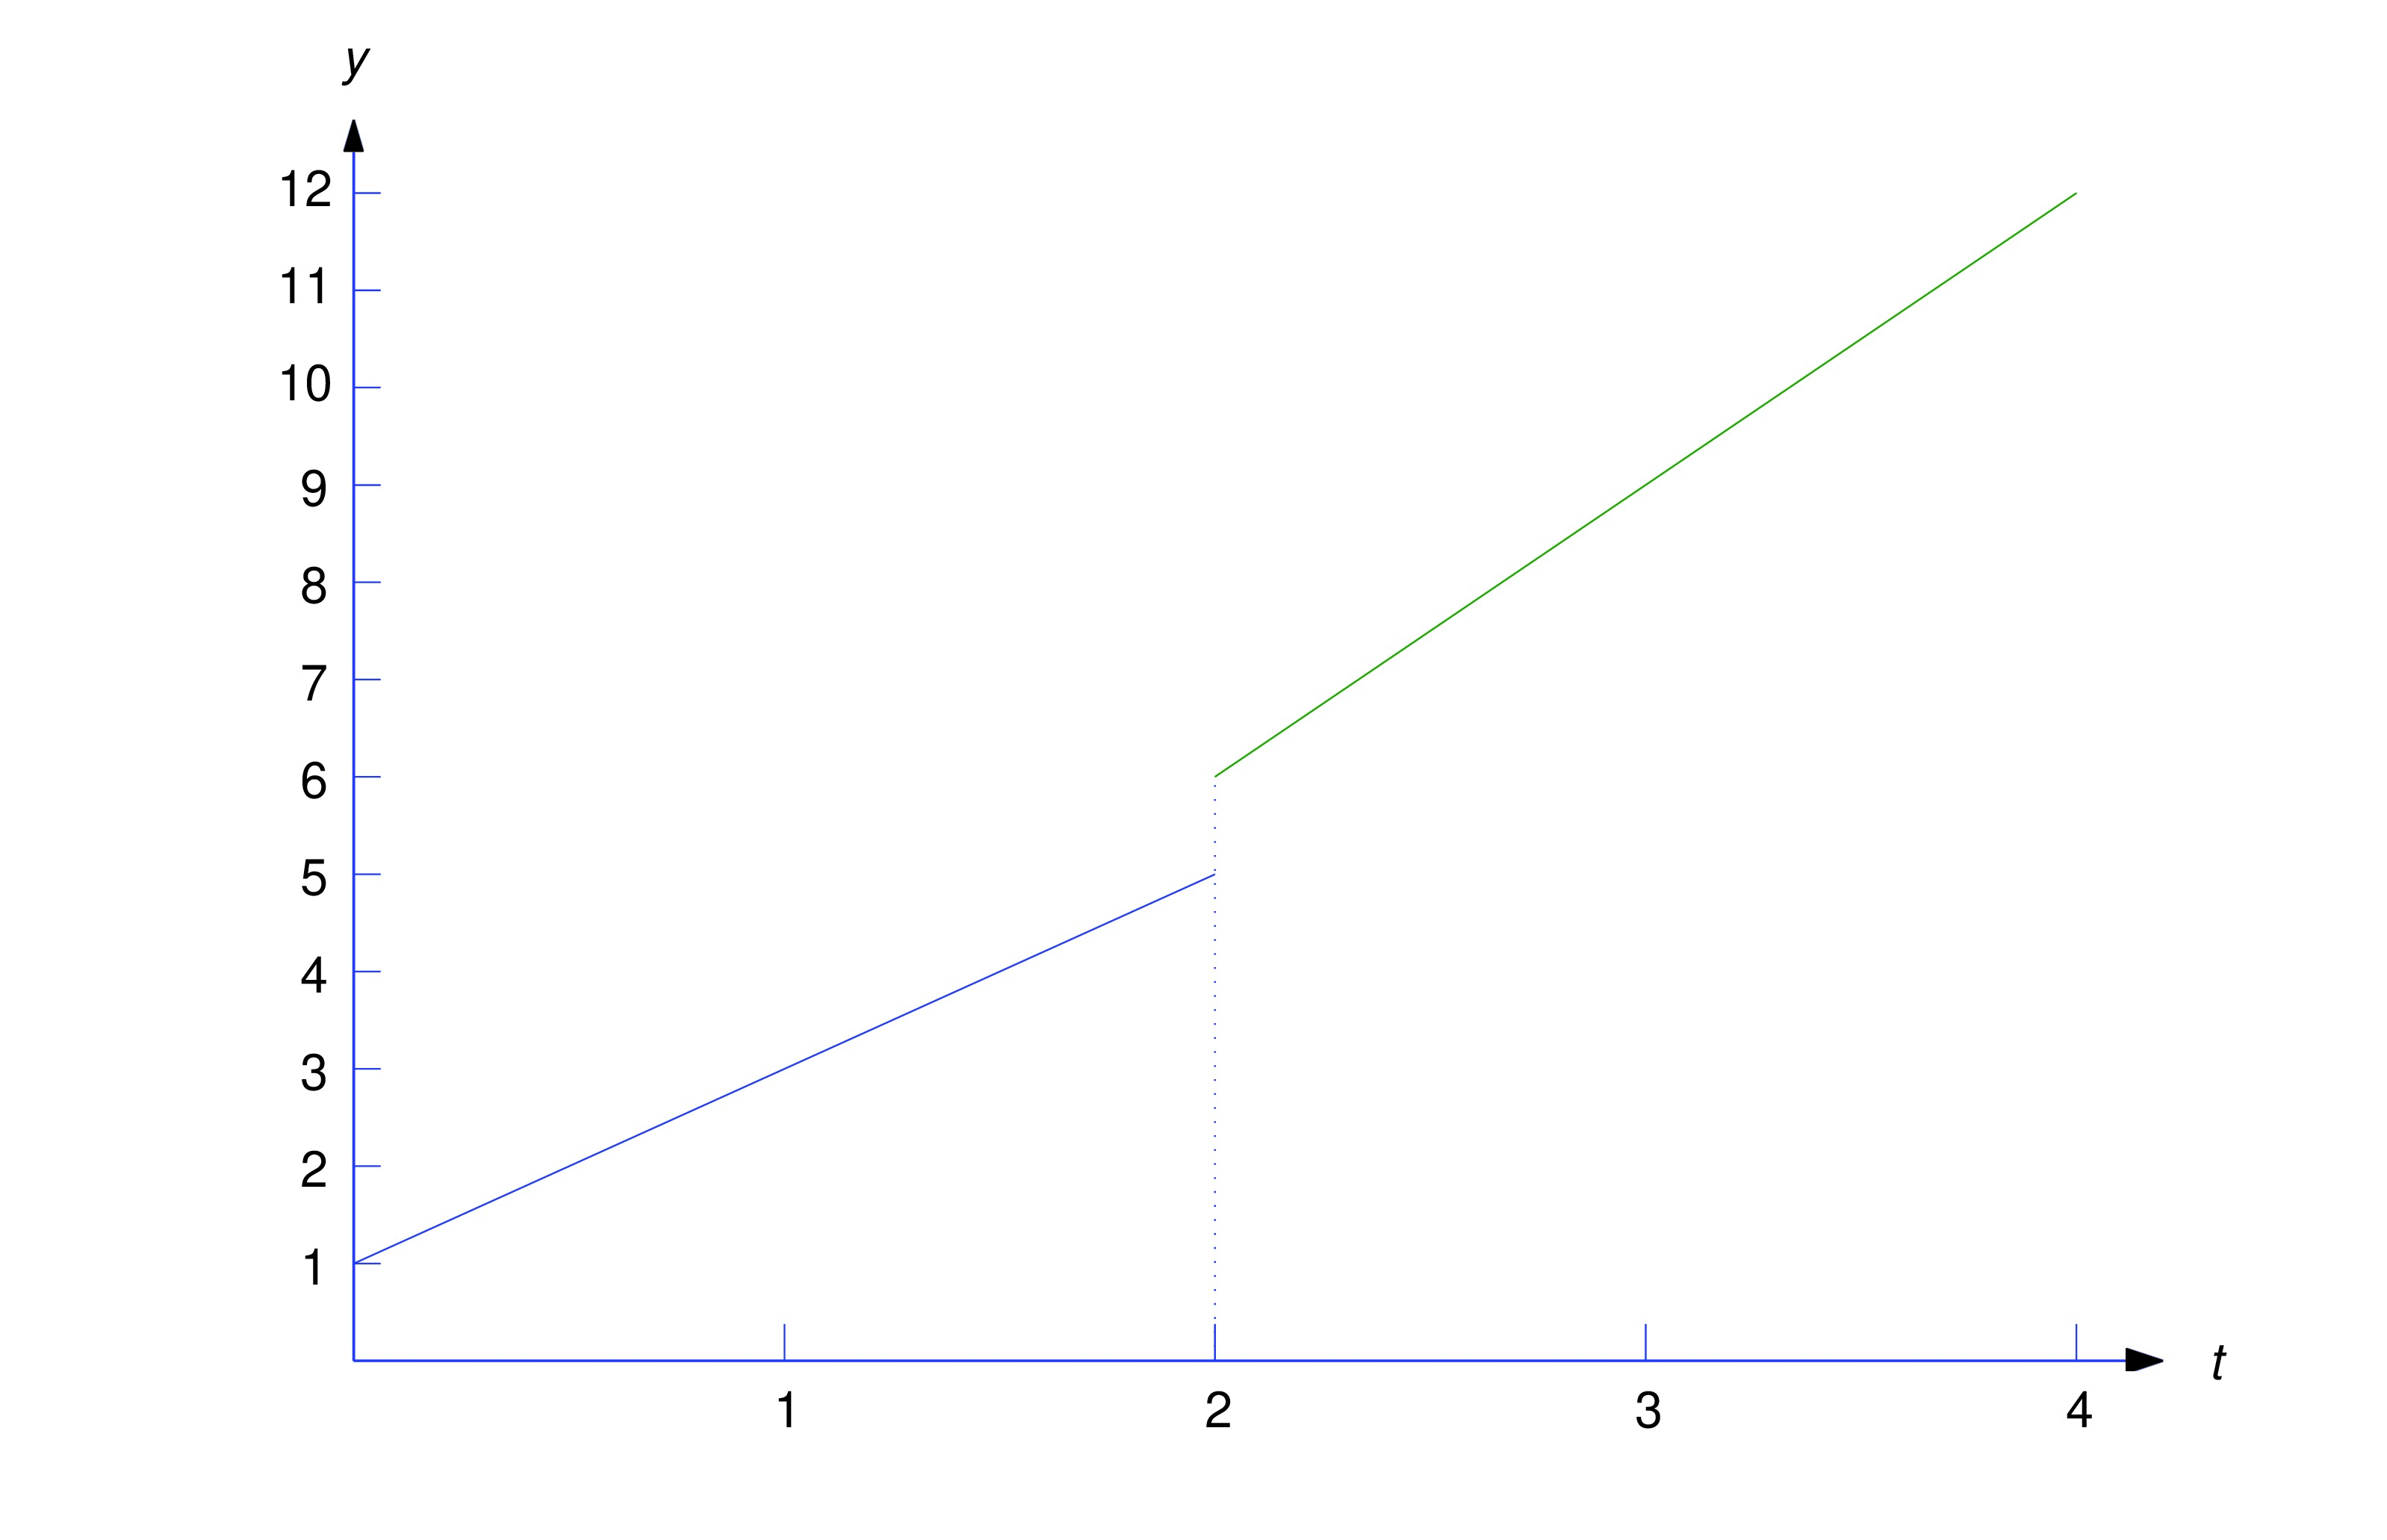
\includegraphics[height=1.5in]{fig080401.jpg}
 \end{image}

\begin{explanation}
Since the formula for $f$ changes at $t=2$, we write
\begin{equation}\label{eq:8.4.2}
\begin{array}{ccl}
{\cal L}(f)&=&\int_0^\infty e^{-st}f(t)\,dt\\
&=&\int_0^2 e^{-st}(2t+1)\,dt+\int_2^\infty e^{-st}(3t)\,dt.
\end{array}
\end{equation}
To relate the first term to a Laplace transform,  we add and subtract
$$
\int_2^\infty e^{-st}(2t+1)\,dt
$$
in \eqref{eq:8.4.2} to obtain
\begin{equation}\label{eq:8.4.3}
\begin{array}{ccl}
{\cal L}(f)&=&\int_0^\infty e^{-st}(2t+1)\,dt+
\int_2^\infty e^{-st}(3t-2t-1)\,dt\\
&=&\int_0^\infty e^{-st}(2t+1)\,dt+
\int_2^\infty e^{-st}(t-1)\,dt\\
&=&{\cal L}(2t+1)+\int_2^\infty e^{-st}(t-1)\,dt.
\end{array}
\end{equation}
To relate the last integral to a Laplace transform,
  we make the change of variable
 $x=t-2$ and rewrite the integral as
\begin{eqnarray*}
\int_2^\infty e^{-st}(t-1)\,dt&=&\int_0^\infty e^{-s(x+2)}(x+1)\,dx
\\
&=&e^{-2s}\int_0^\infty e^{-sx}(x+1)\,dx.
\end{eqnarray*}
Since the symbol used for the variable of integration has no effect on the
value of a definite integral, we can now replace $x$ by the more standard
$t$ and write
$$
\int_2^\infty e^{-st}(t-1)\,dt
=e^{-2s}\int_0^\infty e^{-st}(t+1)\,dt=e^{-2s}{\cal L}(t+1).
$$
This and \eqref{eq:8.4.3} imply that
$$
{\cal L}(f)={\cal L}(2t+1)+e^{-2s}{\cal L} (t+1).
$$
Now we can use the table of Laplace transforms to find that
$$
{\cal L}(f)=\frac{2}{s^2}+\frac{1}{s} +e^{-2s}\left(\frac{1}{s^2}+\frac{1}{s}\right).
$$
\end{explanation}
\end{example}

% \begin{figure}[H]
% \color{blue}
%   \begin{minipage}[b]{0.5\linewidth}
%     \centering
%   \scalebox{.65}{
%   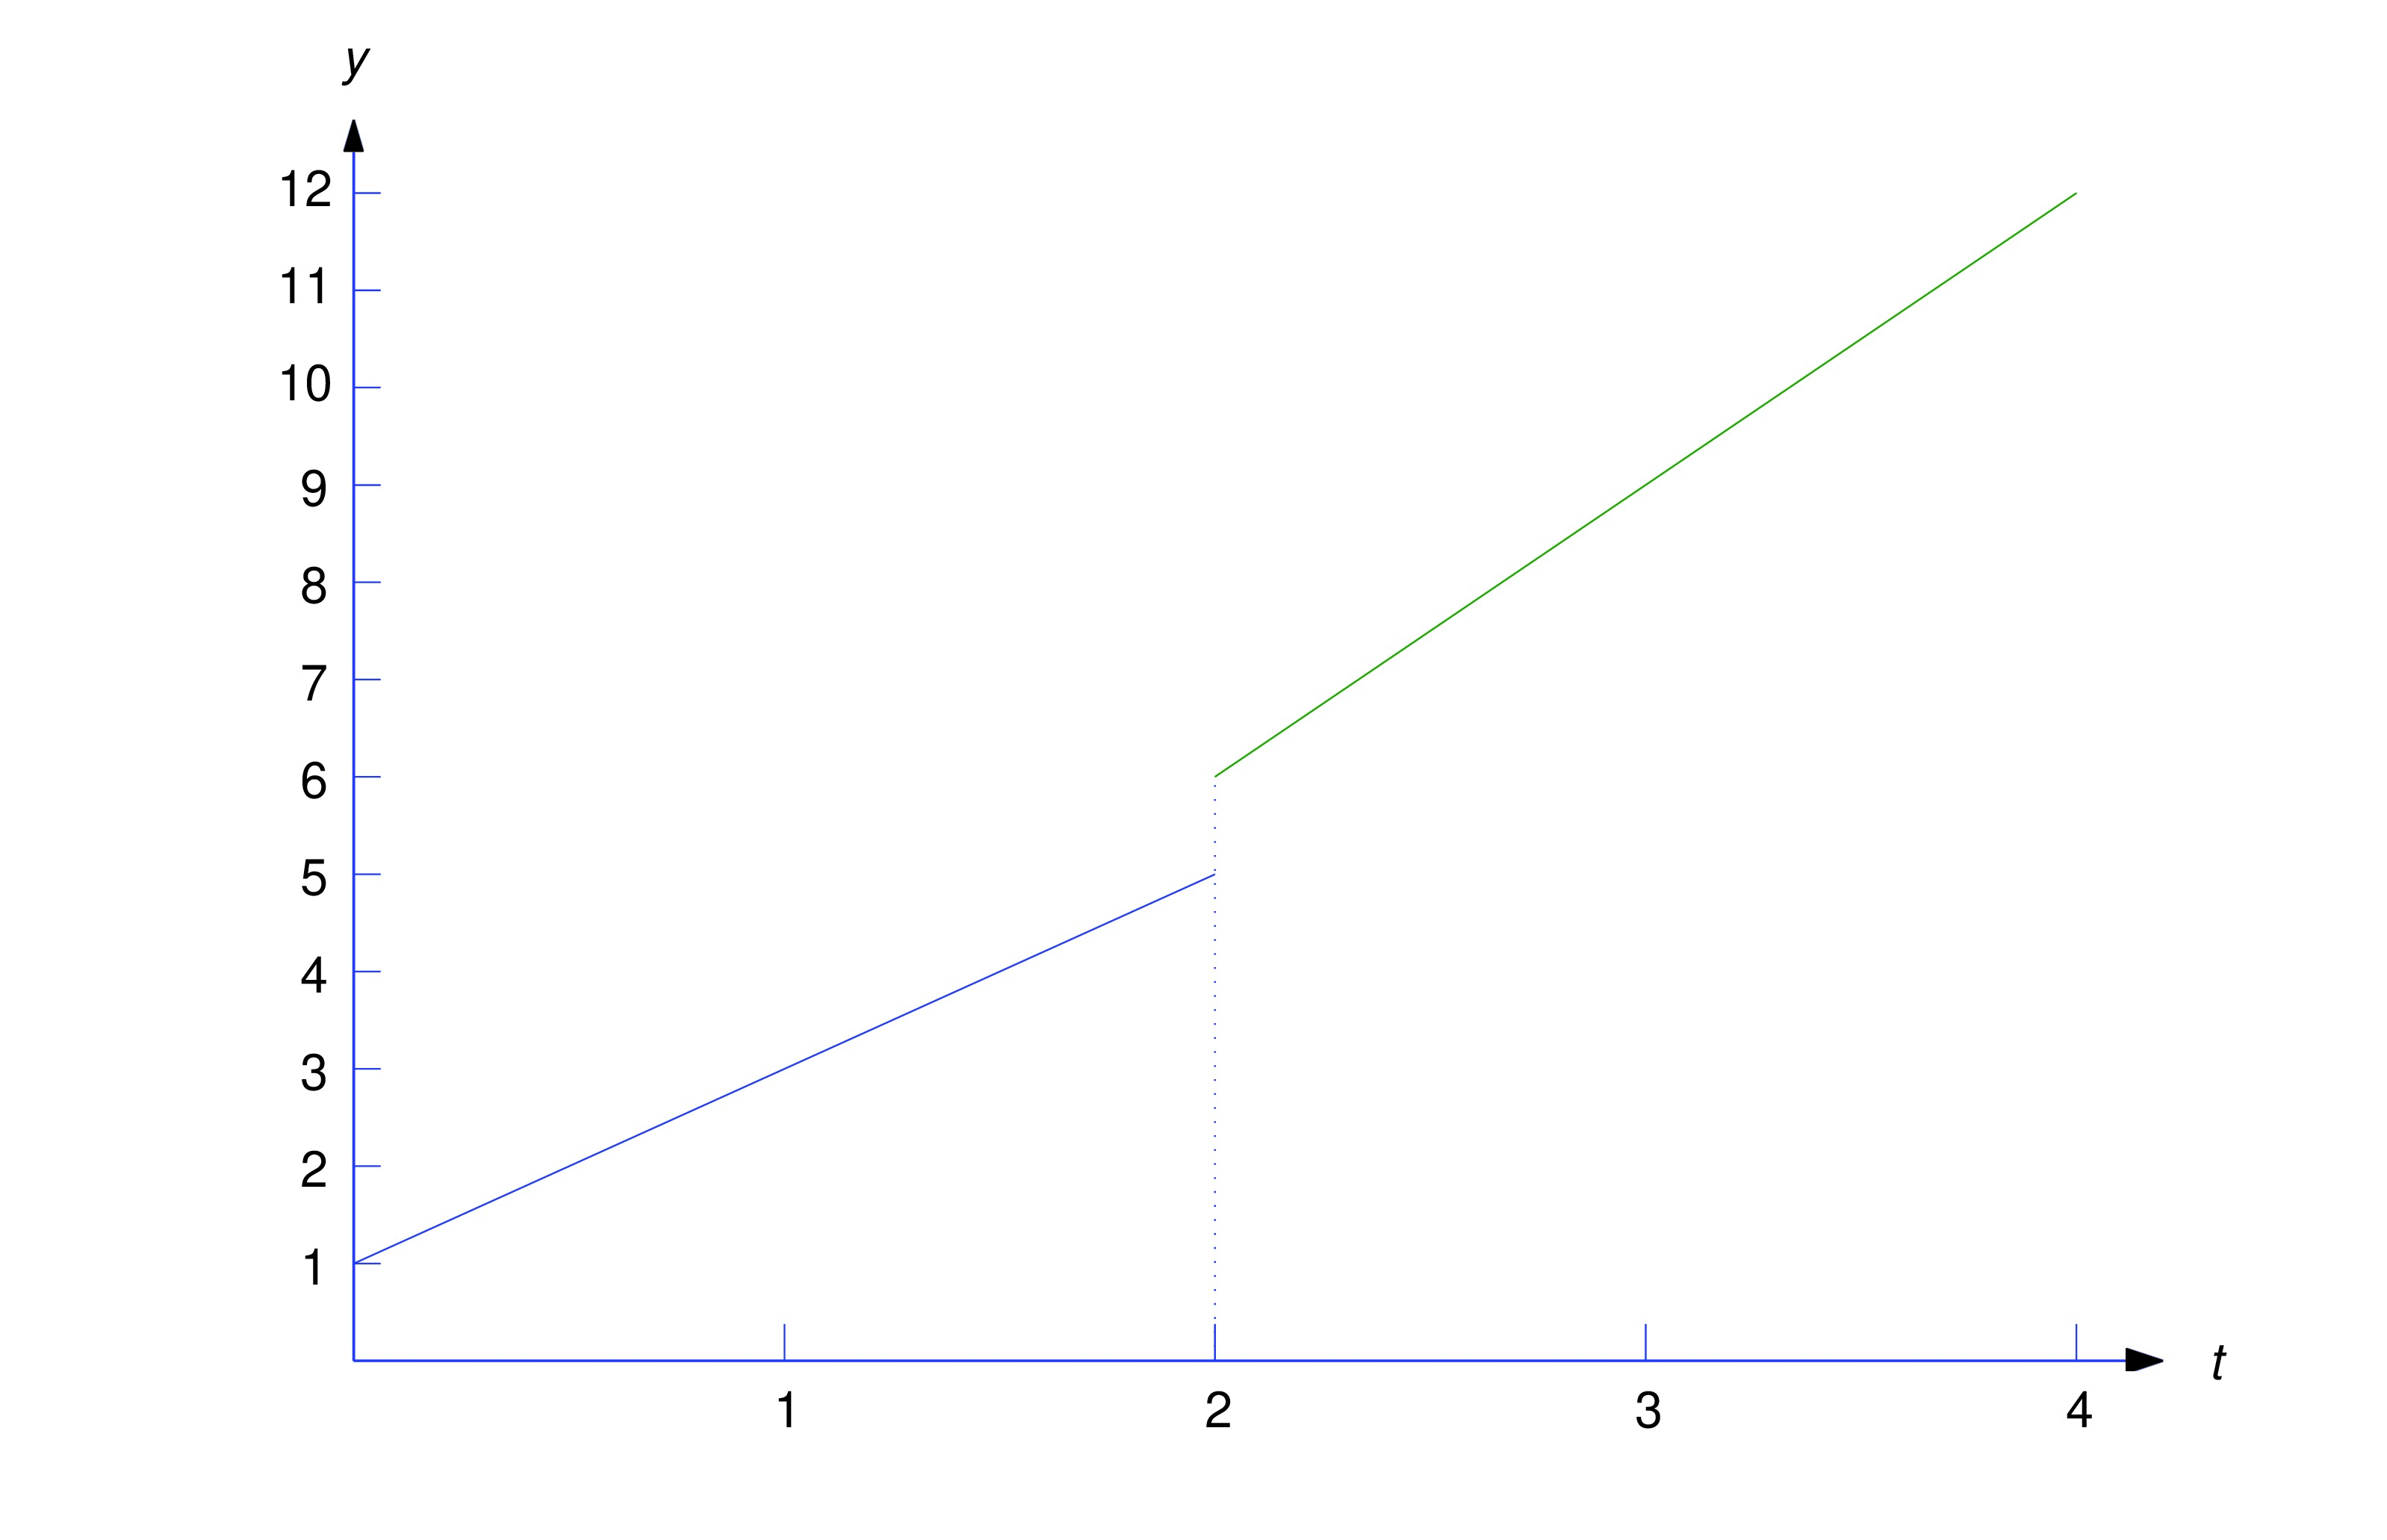
\includegraphics[bb=-78 148 689 643,width=5.67in,height=3.66in,keepaspectratio]{fig080401}}
% \caption{The piecewise
%  continuous function \eqref{eq:8.4.1}}
%   \label{figure:8.4.1}
% \end{minipage}
%   \begin{minipage}[b]{0.5\linewidth}
%     \centering
%   \scalebox{.65}{
%   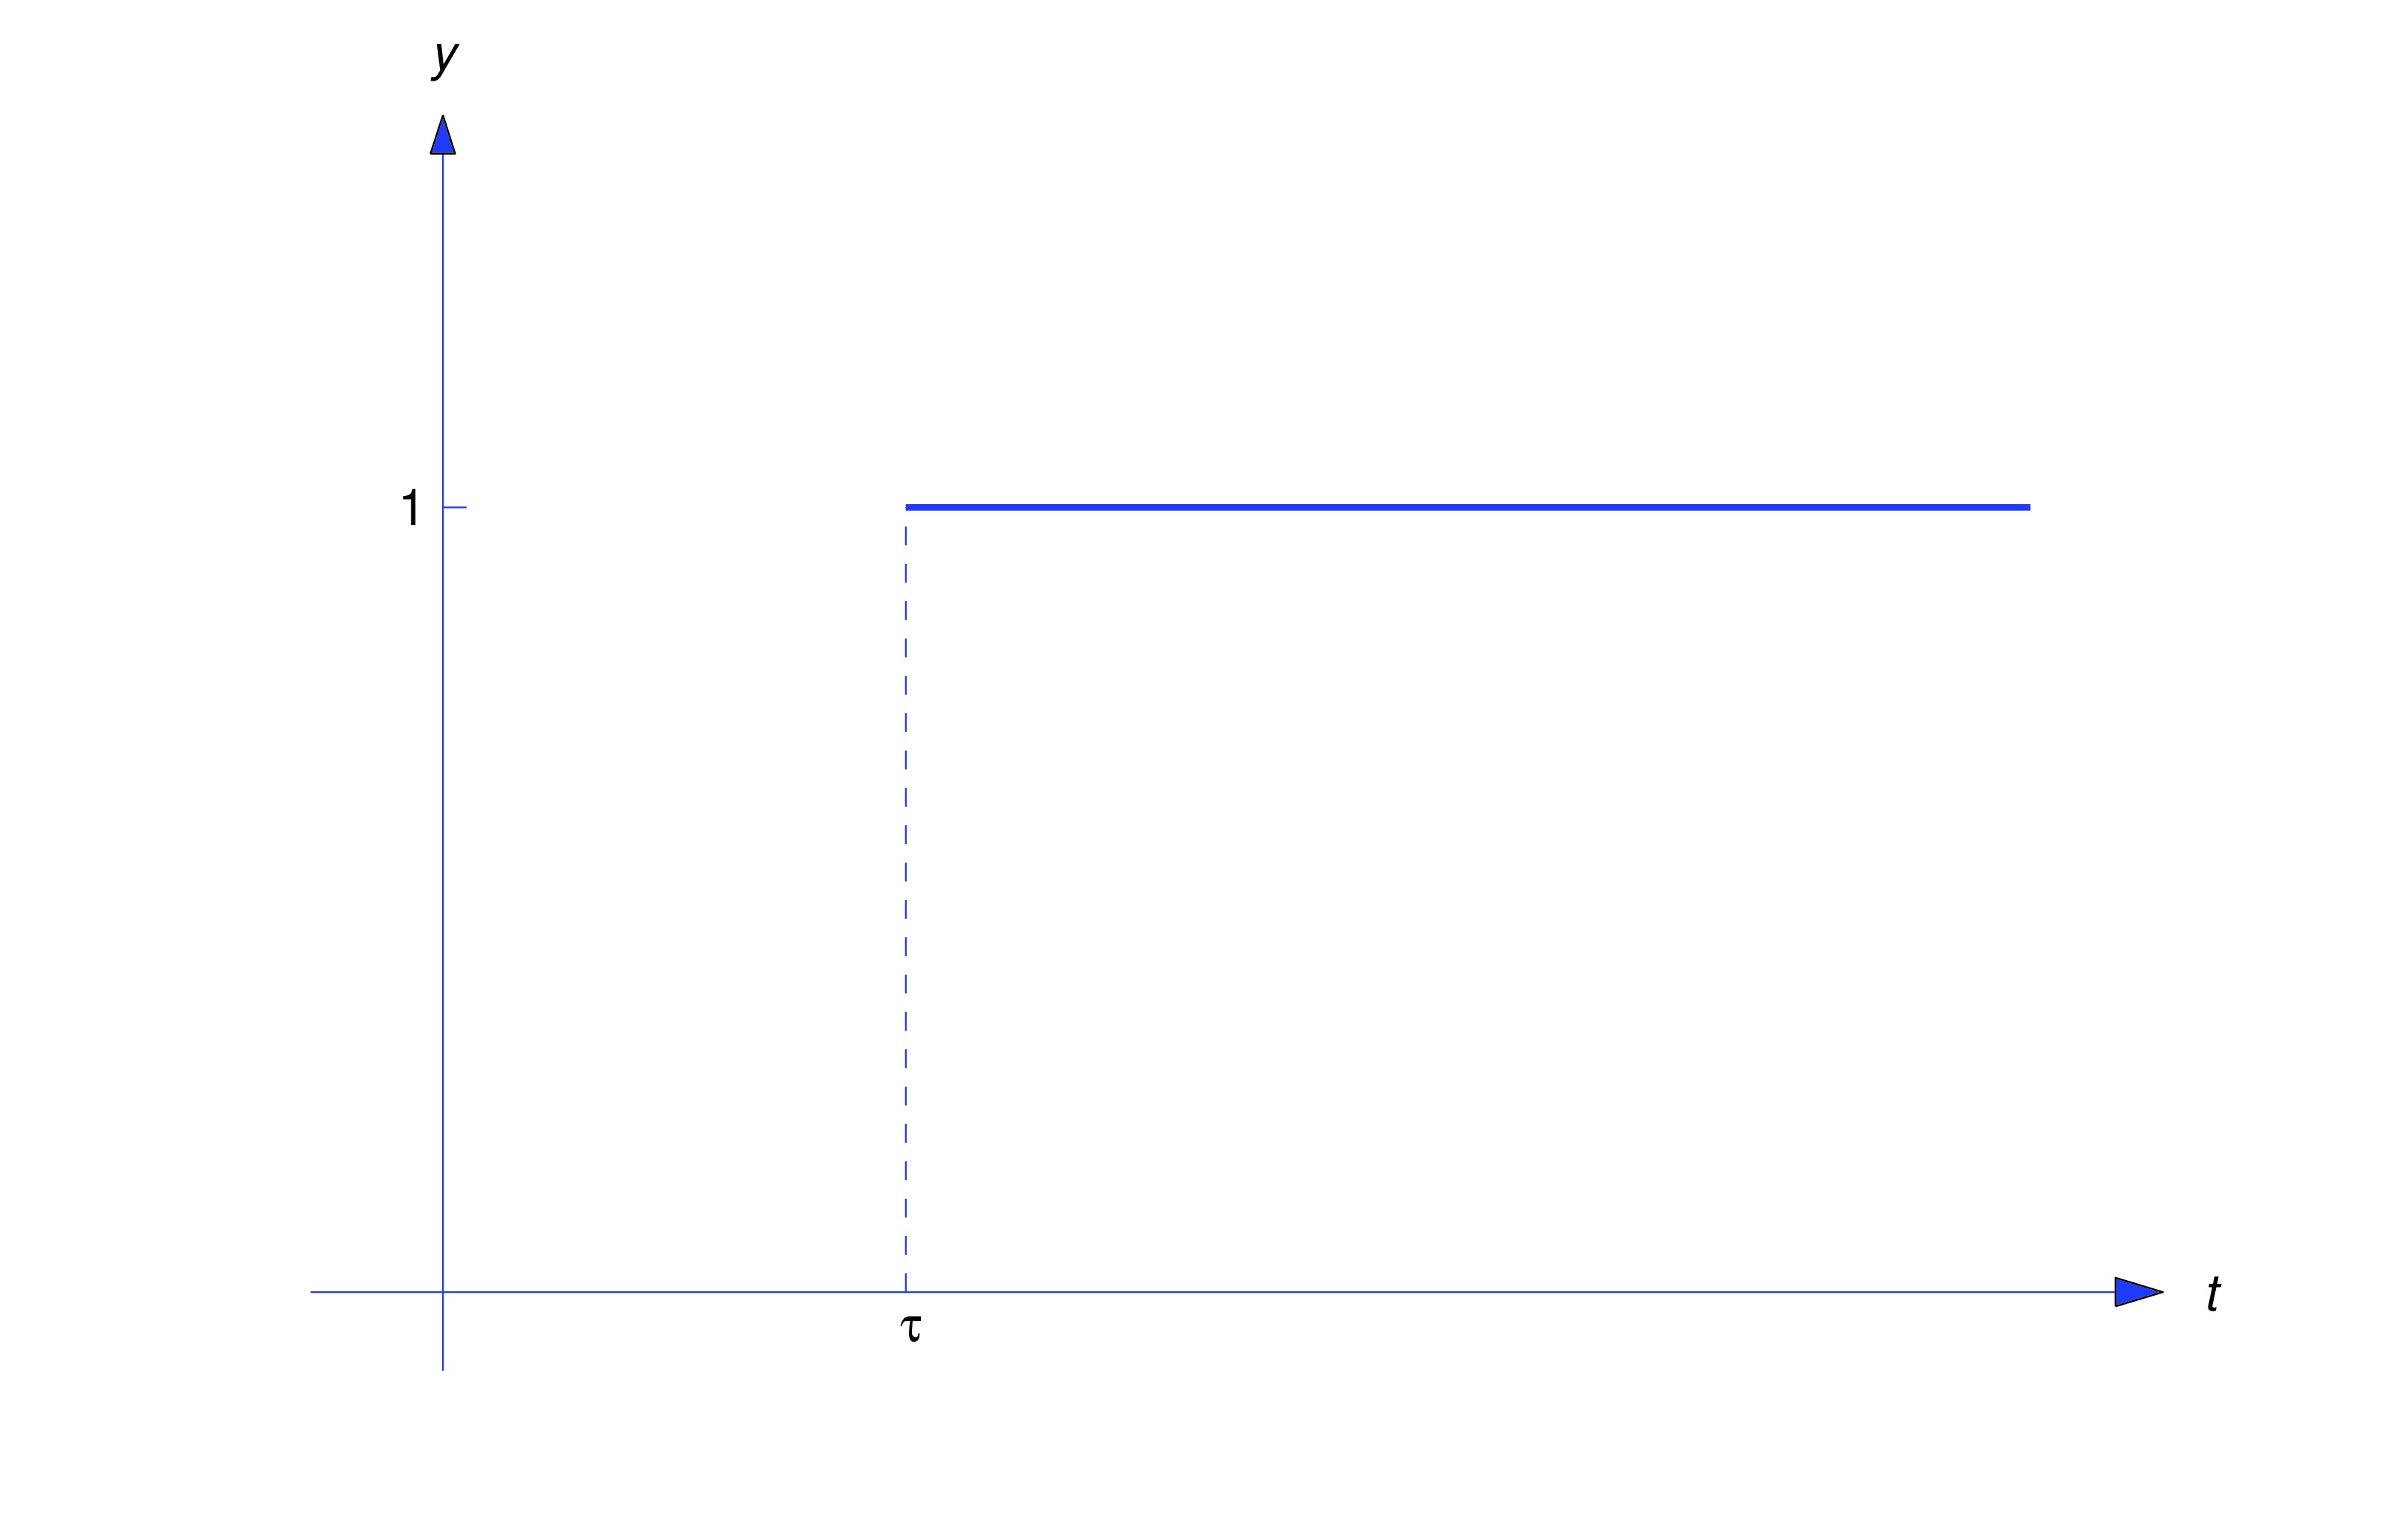
\includegraphics[bb=-78 148 689 643,width=5.67in,height=3.66in,keepaspectratio]{fig080402}}
% \caption{ $y=u(t-\tau)$}
%   \label{figure:8.4.2}
% \end{minipage}
% \end{figure}

\subsection*{Laplace Transforms of Piecewise Continuous Functions}

We'll now develop the method of Example~\ref{example:8.4.1} into a
systematic way to find the Laplace transform of a piecewise continuous
function. It is convenient to introduce the \textit{unit step
function}, defined as
\begin{equation}\label{eq:8.4.4}
u(t)=\left\{\begin{array}{rl}
0,&t<0\\
1,&t\geq 0.
\end{array}\right.
\end{equation}
Thus, $u(t)$ ``steps'' from the constant value $0$ to the constant
value $1$ at $t=0$. If we replace $t$ by
$t-\tau$ in \eqref{eq:8.4.4}, then
$$
u(t-\tau)=\left\{\begin{array}{rl}
0,&t<\tau,\\
1,&t\geq \tau
\end{array}\right.;
$$
that is, the step now occurs at $t=\tau$ (See figure below) %(Figure~\ref{figure:8.4.2}).

\begin{image}
 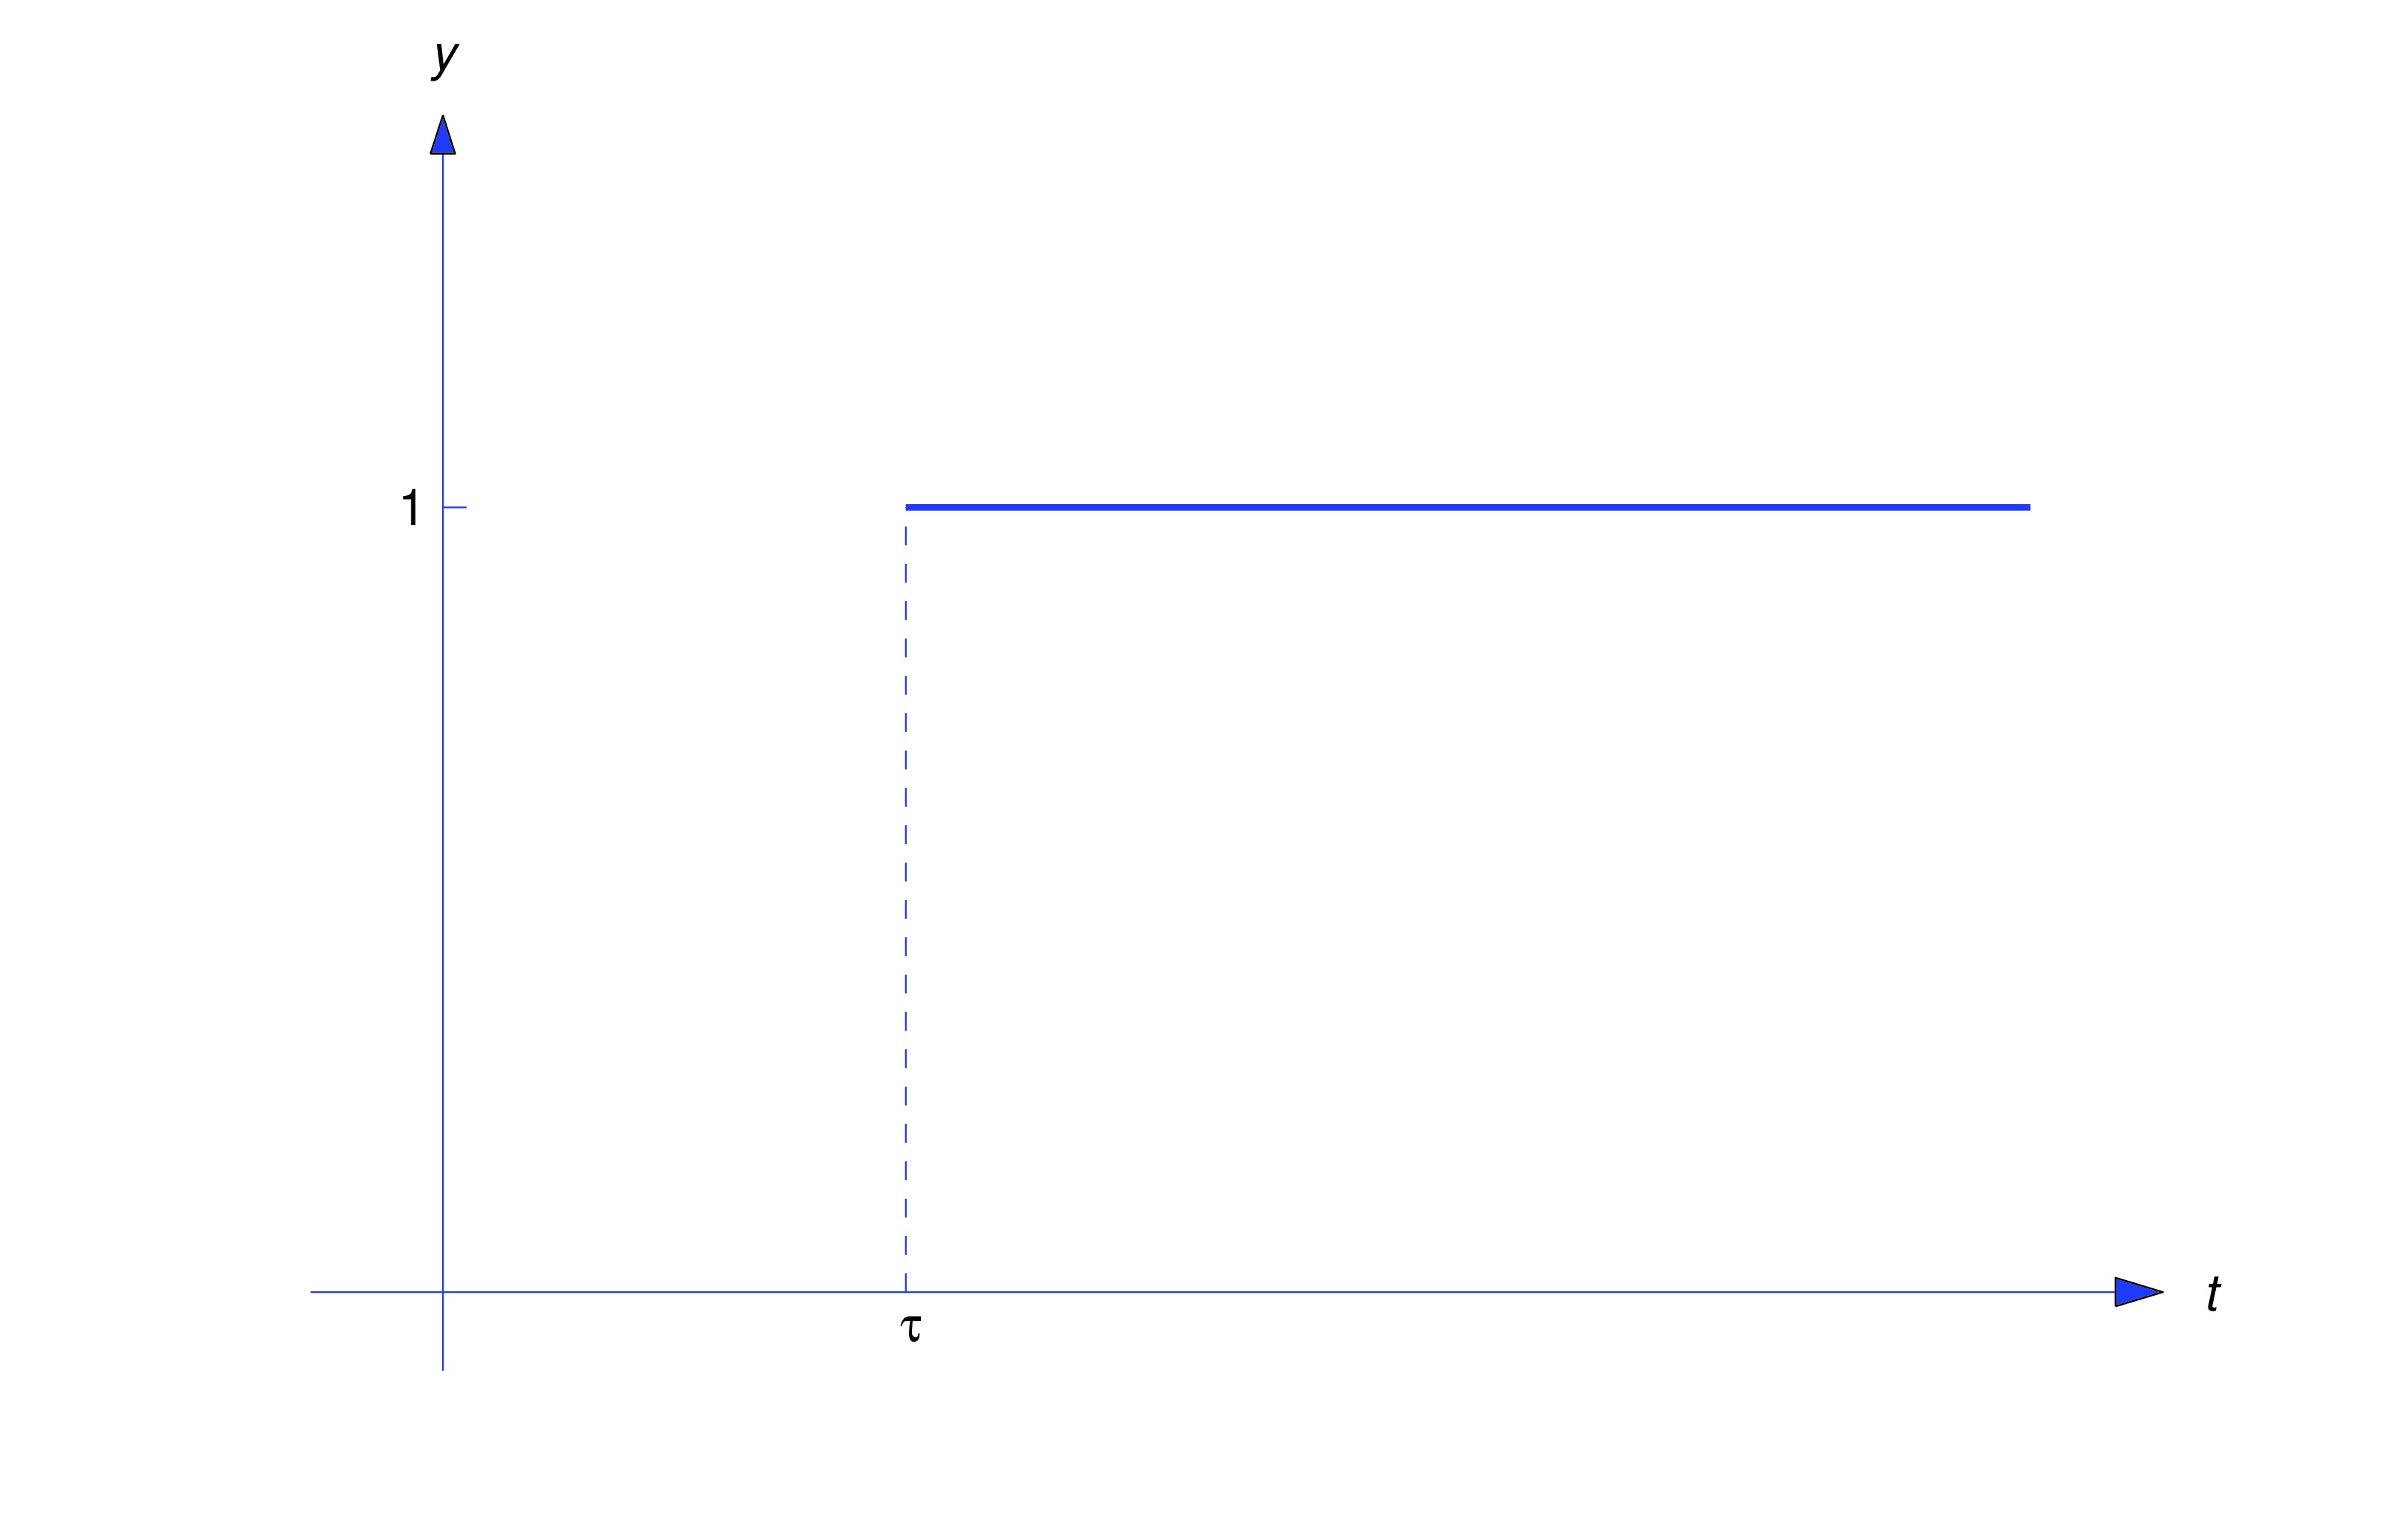
\includegraphics[height=1.5in]{fig080402.jpg}
\end{image}

The step function enables us to represent piecewise continuous
functions conveniently. For example, consider the function
\begin{equation}\label{eq:8.4.5}
f(t)=\left\{\begin{array}{rl}
f_0(t),&0\leq t<t_1,\\
f_1(t),&t\geq t_1,
\end{array}\right.
\end{equation}
where we assume that $f_0$ and $f_1$ are defined on $[0,\infty)$, even
though they equal $f$ only on the indicated intervals. This assumption
enables us to rewrite \eqref{eq:8.4.5} as
\begin{equation}\label{eq:8.4.6}
f(t)=f_0(t)+u(t-t_1)\left(f_1(t)-f_0(t)\right).
\end{equation}
To verify this, note that if $t<t_1$ then $u(t-t_1)=0$ and
\eqref{eq:8.4.6}  becomes
$$
f(t)=f_0(t)+(0)\left(f_1(t)-f_0(t)\right)=f_0(t).
$$
If $t\geq t_1$ then $u(t-t_1)=1$ and  \eqref{eq:8.4.6} becomes
$$
f(t)=f_0(t)+(1)\left(f_1(t)-f_0(t)\right)=f_1(t).
$$

We need the next theorem to
 show how \eqref{eq:8.4.6} can be used to find ${\cal L}(f)$.

\begin{theorem}\label{thmtype:8.4.1}
Let $g$ be defined on $[0,\infty).$ Suppose   $\tau\geq 0$ and ${\cal
L}\left(g(t+\tau)\right)$ exists for $s>s_0.$ Then ${\cal
L}\left(u(t-\tau)g(t)\right)$ exists for $s>s_0$, and
$$
{\cal L}(u(t-\tau)g(t))=e^{-s\tau}{\cal L}\left(g(t+\tau)\right).
$$
\end{theorem}

\begin{proof}
By definition,
$$
{\cal L}\left(u(t-\tau)g(t)\right)=\int_0^\infty e^{-st} u(t-\tau)g(t)\,
dt.
$$
From this and the definition of $u(t-\tau)$,
$$
{\cal L}\left(u(t-\tau)g(t)\right)=\int_0^\tau
e^{-st}(0)\,dt+\int_{\tau}^\infty e^{-st}g(t)\,dt.
$$
The first integral on the right equals zero.  Introducing the new variable
of integration $x=t-\tau$ in the second integral yields
$$
{\cal L}\left(u(t-\tau)g(t)\right)=\int_0^\infty e^{-s(x+\tau)}g(x+\tau)\,dx
=e^{-s\tau}\int_0^\infty e^{-sx} g(x+\tau)\,dx.
$$
Changing the name of the variable of integration in the last integral
from $x$ to $t$ yields
$$
{\cal L}\left(u(t-\tau)g(t)\right)
=e^{-s\tau}\int_0^\infty e^{-st} g(t+\tau)\,dt=e^{-s\tau}{\cal
L}(g(t+\tau)).
$$
\end{proof}

\begin{example}\label{example:8.4.2}
 Find
$$
{\cal L}\left(u(t-1)(t^2+1)\right).
$$
\begin{explanation}
Here $\tau=1$ and $g(t)=t^2+1$, so
$$
g(t+1)=(t+1)^2+1=t^2+2t+2.
$$
Since
$$
{\cal L}\left(g(t+1)\right)=\frac{2}{s^3}+\frac{2}{s^2}+\frac{2}{s},
$$
Theorem~\ref{thmtype:8.4.1} implies that
$${\cal L}\left(u(t-1)(t^2+1)\right)
=e^{-s}\left(\frac{2}{s^3}+\frac{2}{s^2}+\frac{2}{s}\right).
$$
\end{explanation}
\end{example}

\begin{example}\label{example:8.4.3}
Use Theorem~\ref{thmtype:8.4.1} to find the Laplace transform of the
function
$$
f(t)=\left\{\begin{array}{cl} 2t+1,&0\leq t<2,\\ 3t,&t\geq 2,
\end{array}\right.
$$
from Example~\ref{example:8.4.1}.


\begin{explanation}
We first write $f$ in the form \eqref{eq:8.4.6} as
$$
f(t)=2t+1+u(t-2)(t-1).
$$
Therefore
\begin{eqnarray*}
{\cal L}(f)&=&{\cal L}(2t+1) +{\cal L}\left(u(t-2)(t-1)\right)\\
&=&{\cal L}(2t+1) +e^{-2s}{\cal L}(t+1)\quad\mbox{ (from
Theorem~\ref{thmtype:8.4.1}})\\
&=&\frac{2}{s^2}+\frac{1}{s}+e^{-2s}\left(\frac{1}{s^2}+\frac{1}{s}\right),
\end{eqnarray*}
which is the result obtained in Example~\ref{example:8.4.1}.

Formula \eqref{eq:8.4.6} can be extended to more general piecewise continuous
functions. For example, we can write
$$
f(t)=\left\{\begin{array}{rl}
f_0(t),&0\leq t<t_1,\\
f_1(t),&t_1\leq t<t_2,\\
f_2(t),&t\geq t_2,
\end{array}\right.
$$
as
$$
f(t)=f_0(t)+u(t-t_1)\left(f_1(t)-f_0(t)\right)+
u(t-t_2)\left(f_2(t)-f_1(t)\right)
$$
if $f_0$, $f_1$, and $f_2$ are all defined on $[0,\infty)$.
\end{explanation}
\end{example}

\begin{example}\label{example:8.4.4}
 Find the Laplace transform of
\begin{equation} \label{eq:8.4.7}
f(t)=\left\{\begin{array}{cl}
 1,&0\leq t<2,\\
-2t+1,&2\leq t<3,\\
 3t,&3\leq t<5,\\
 t-1,&t\geq 5
\end{array}\right.
\end{equation}
\begin{image}
 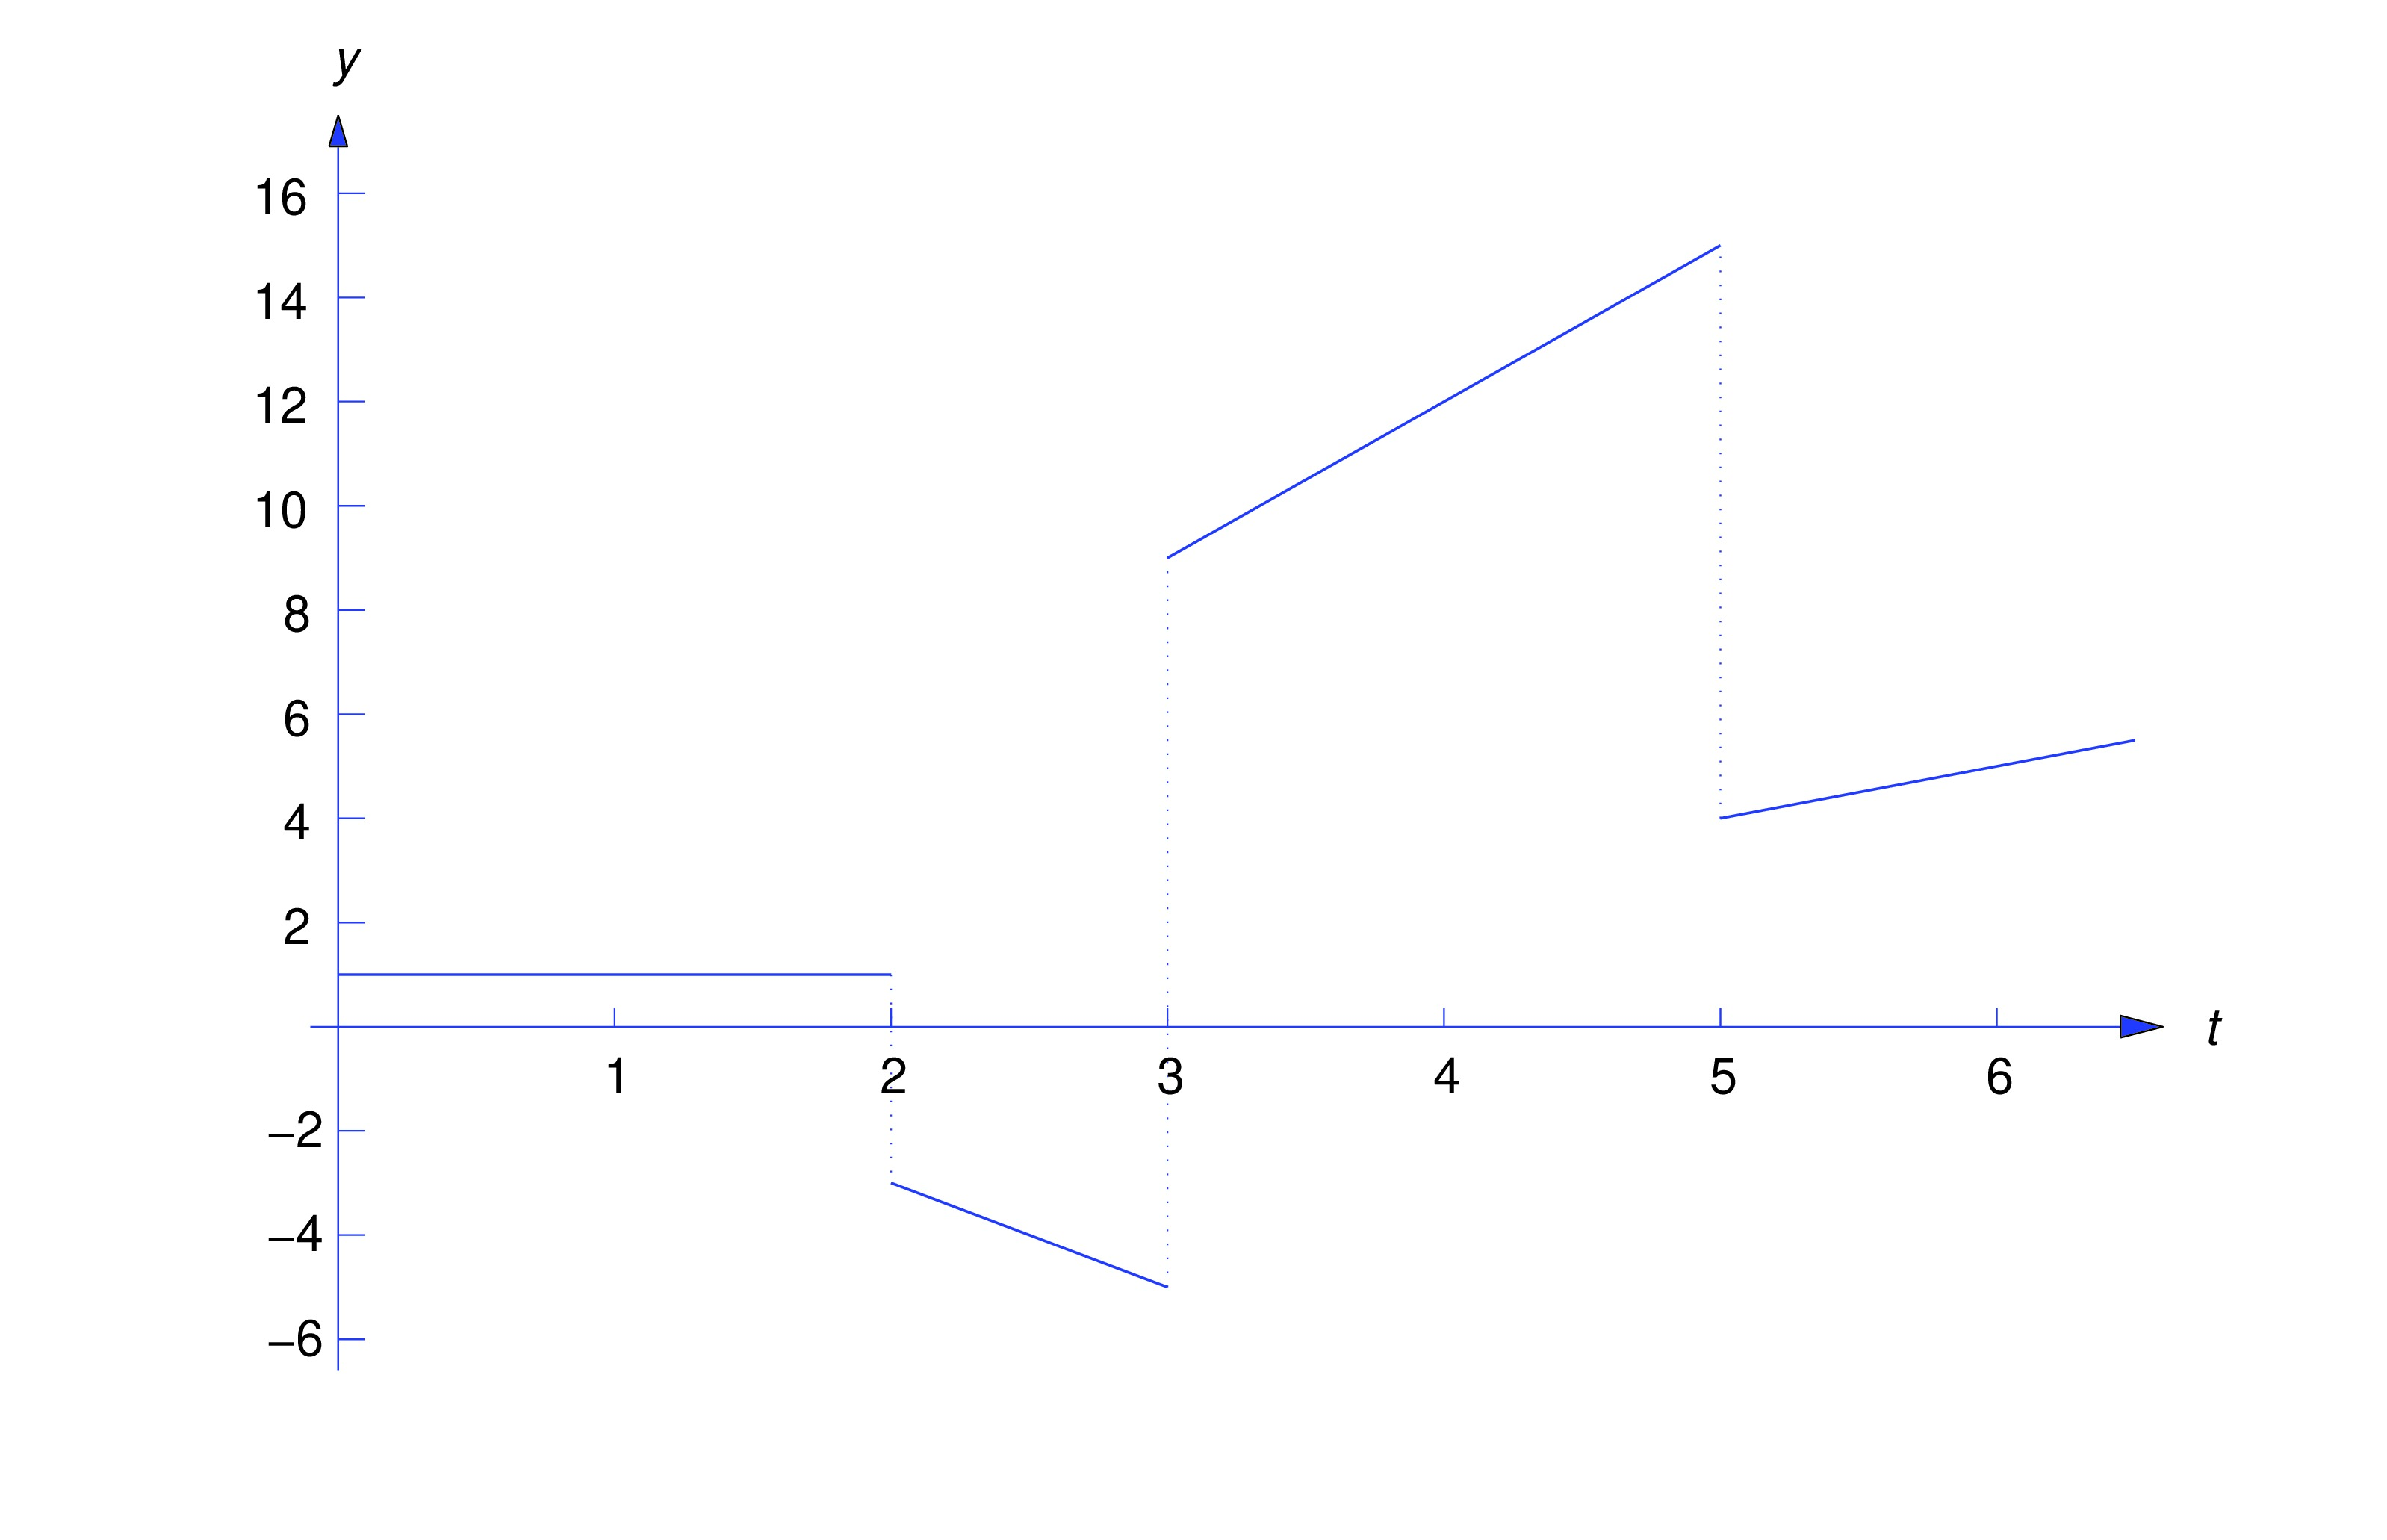
\includegraphics[height=1.5in]{fig080403.jpg}
 \end{image}
%(Figure~\ref{figure:8.4.3}).
\begin{explanation}
In terms of step functions,
\begin{eqnarray*}
f(t)&=&1+u(t-2)(-2t+1-1)+u(t-3)(3t+2t-1)\\
&&+u(t-5)(t-1-3t),
\end{eqnarray*}
or
$$
f(t)=1-2u(t-2)t+u(t-3)(5t-1)-u(t-5)(2t+1).
$$
Now Theorem~\ref{thmtype:8.4.1} implies that
\begin{eqnarray*}
{\cal L}(f)&=&{\cal L}(1)-2e^{-2s}{\cal L}(t+2)+e^{-3s}{\cal
L}\left(5(t+3)-1\right)-e^{-5s}{\cal L}\left(2(t+5)+1\right)\\
&=&{\cal L}(1)-2e^{-2s}{\cal L}(t+2)+e^{-3s}{\cal
L}(5t+14)-e^{-5s}{\cal L}(2t+11)\\
&=&\frac{1}{s}-2e^{-2s}\left(\frac{1}{s^2}+\frac{2}{s}\right)+
e^{-3s}\left(\frac{5}{s^2}+\frac{14}{s}\right)-e^{-5s}\left(\frac{2}{s^2}+\frac{11}{s}\right).
\end{eqnarray*}
\end{explanation}
\end{example}

% \begin{figure}[tbp]
%   \centering\color{blue}
%   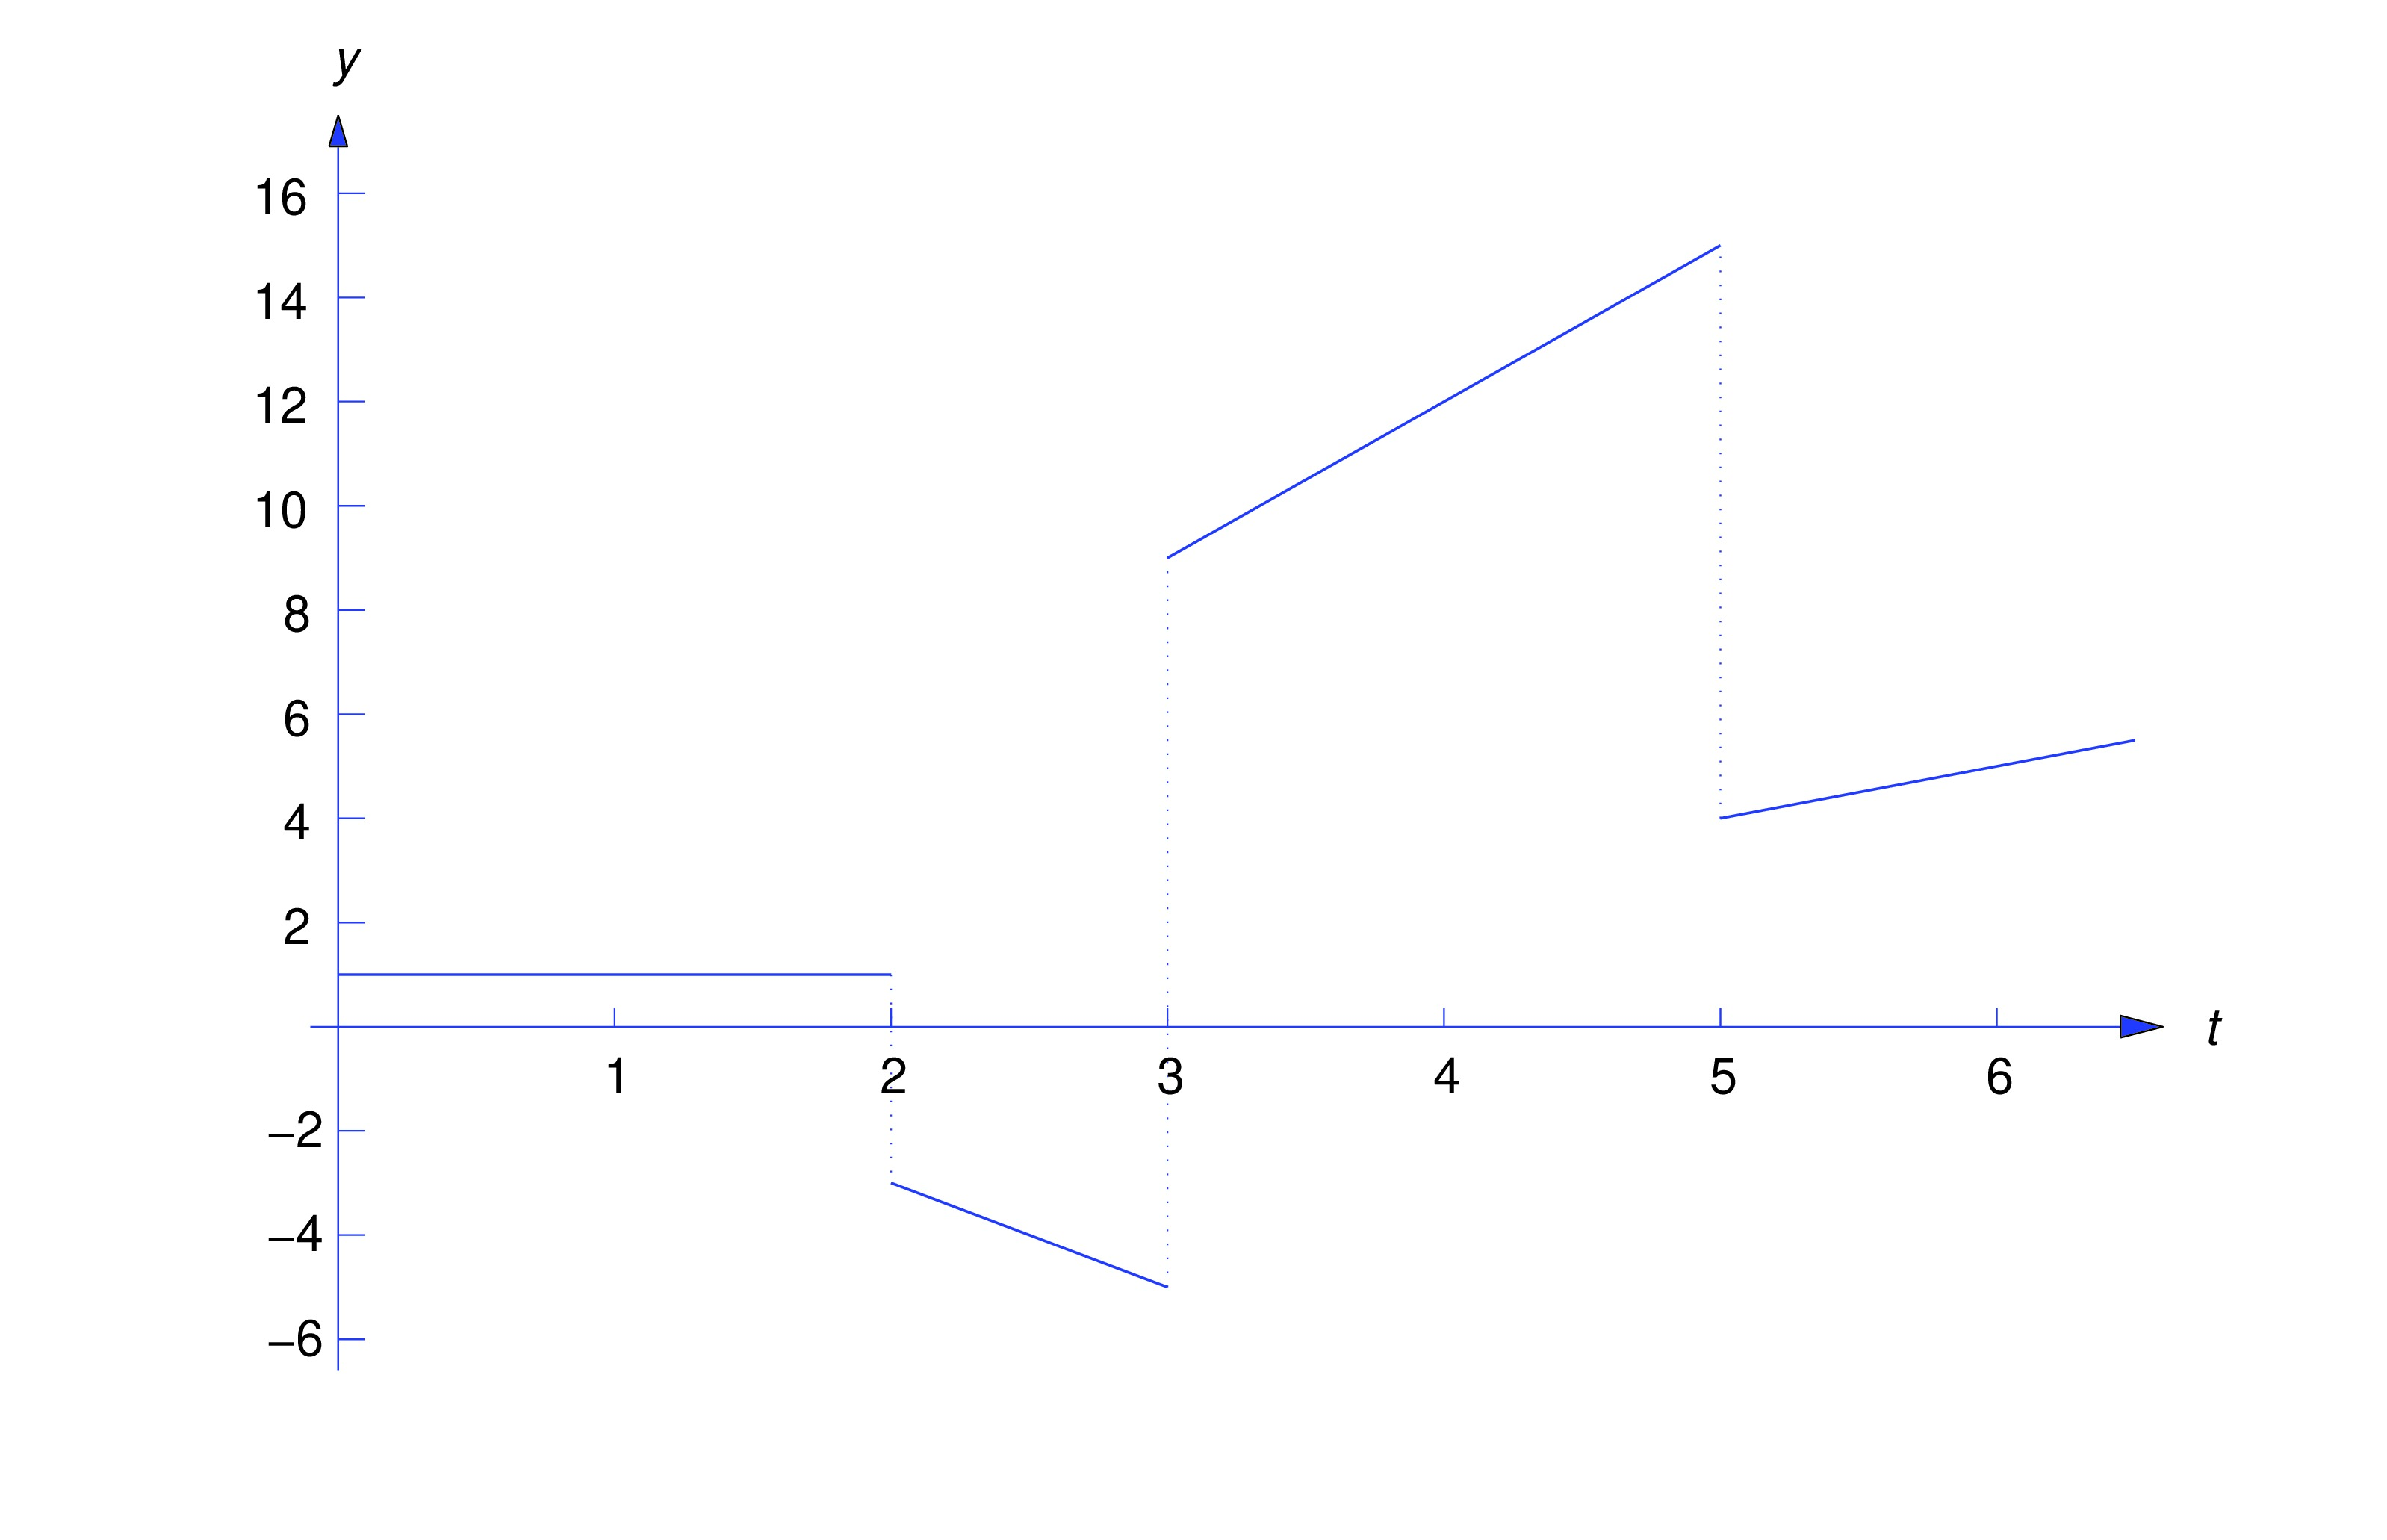
\includegraphics[bb=-78 148 689 643,width=5.67in,height=3.66in,keepaspectratio]{fig080403}
%   \caption{The piecewise contnuous function \eqref{eq:8.4.7}}
%   \label{figure:8.4.3}
% \end{figure}

 The trigonometric identities
\begin{eqnarray}
\sin (A+B)&=&\sin A\cos B+\cos A\sin B\label{eq:8.4.8}\\
\cos (A+B)&=&\cos A\cos B-\sin A\sin B\label{eq:8.4.9}
\end{eqnarray}
are useful in problems that involve shifting the arguments of
trigonometric functions. We'll use these identities in the next
example.

\begin{example}\label{example:8.4.5}
 Find the Laplace transform of
\begin{equation} \label{eq:8.4.10}
f(t)=\left\{\begin{array}{cl}
\sin t,&0\leq t<\frac{\pi}{2},\\
\cos t-3\sin t,&\frac{\pi}{2}\leq t<\pi,\\
 3\cos t,&t\geq\pi
\end{array}\right.
\end{equation}
\begin{image}
 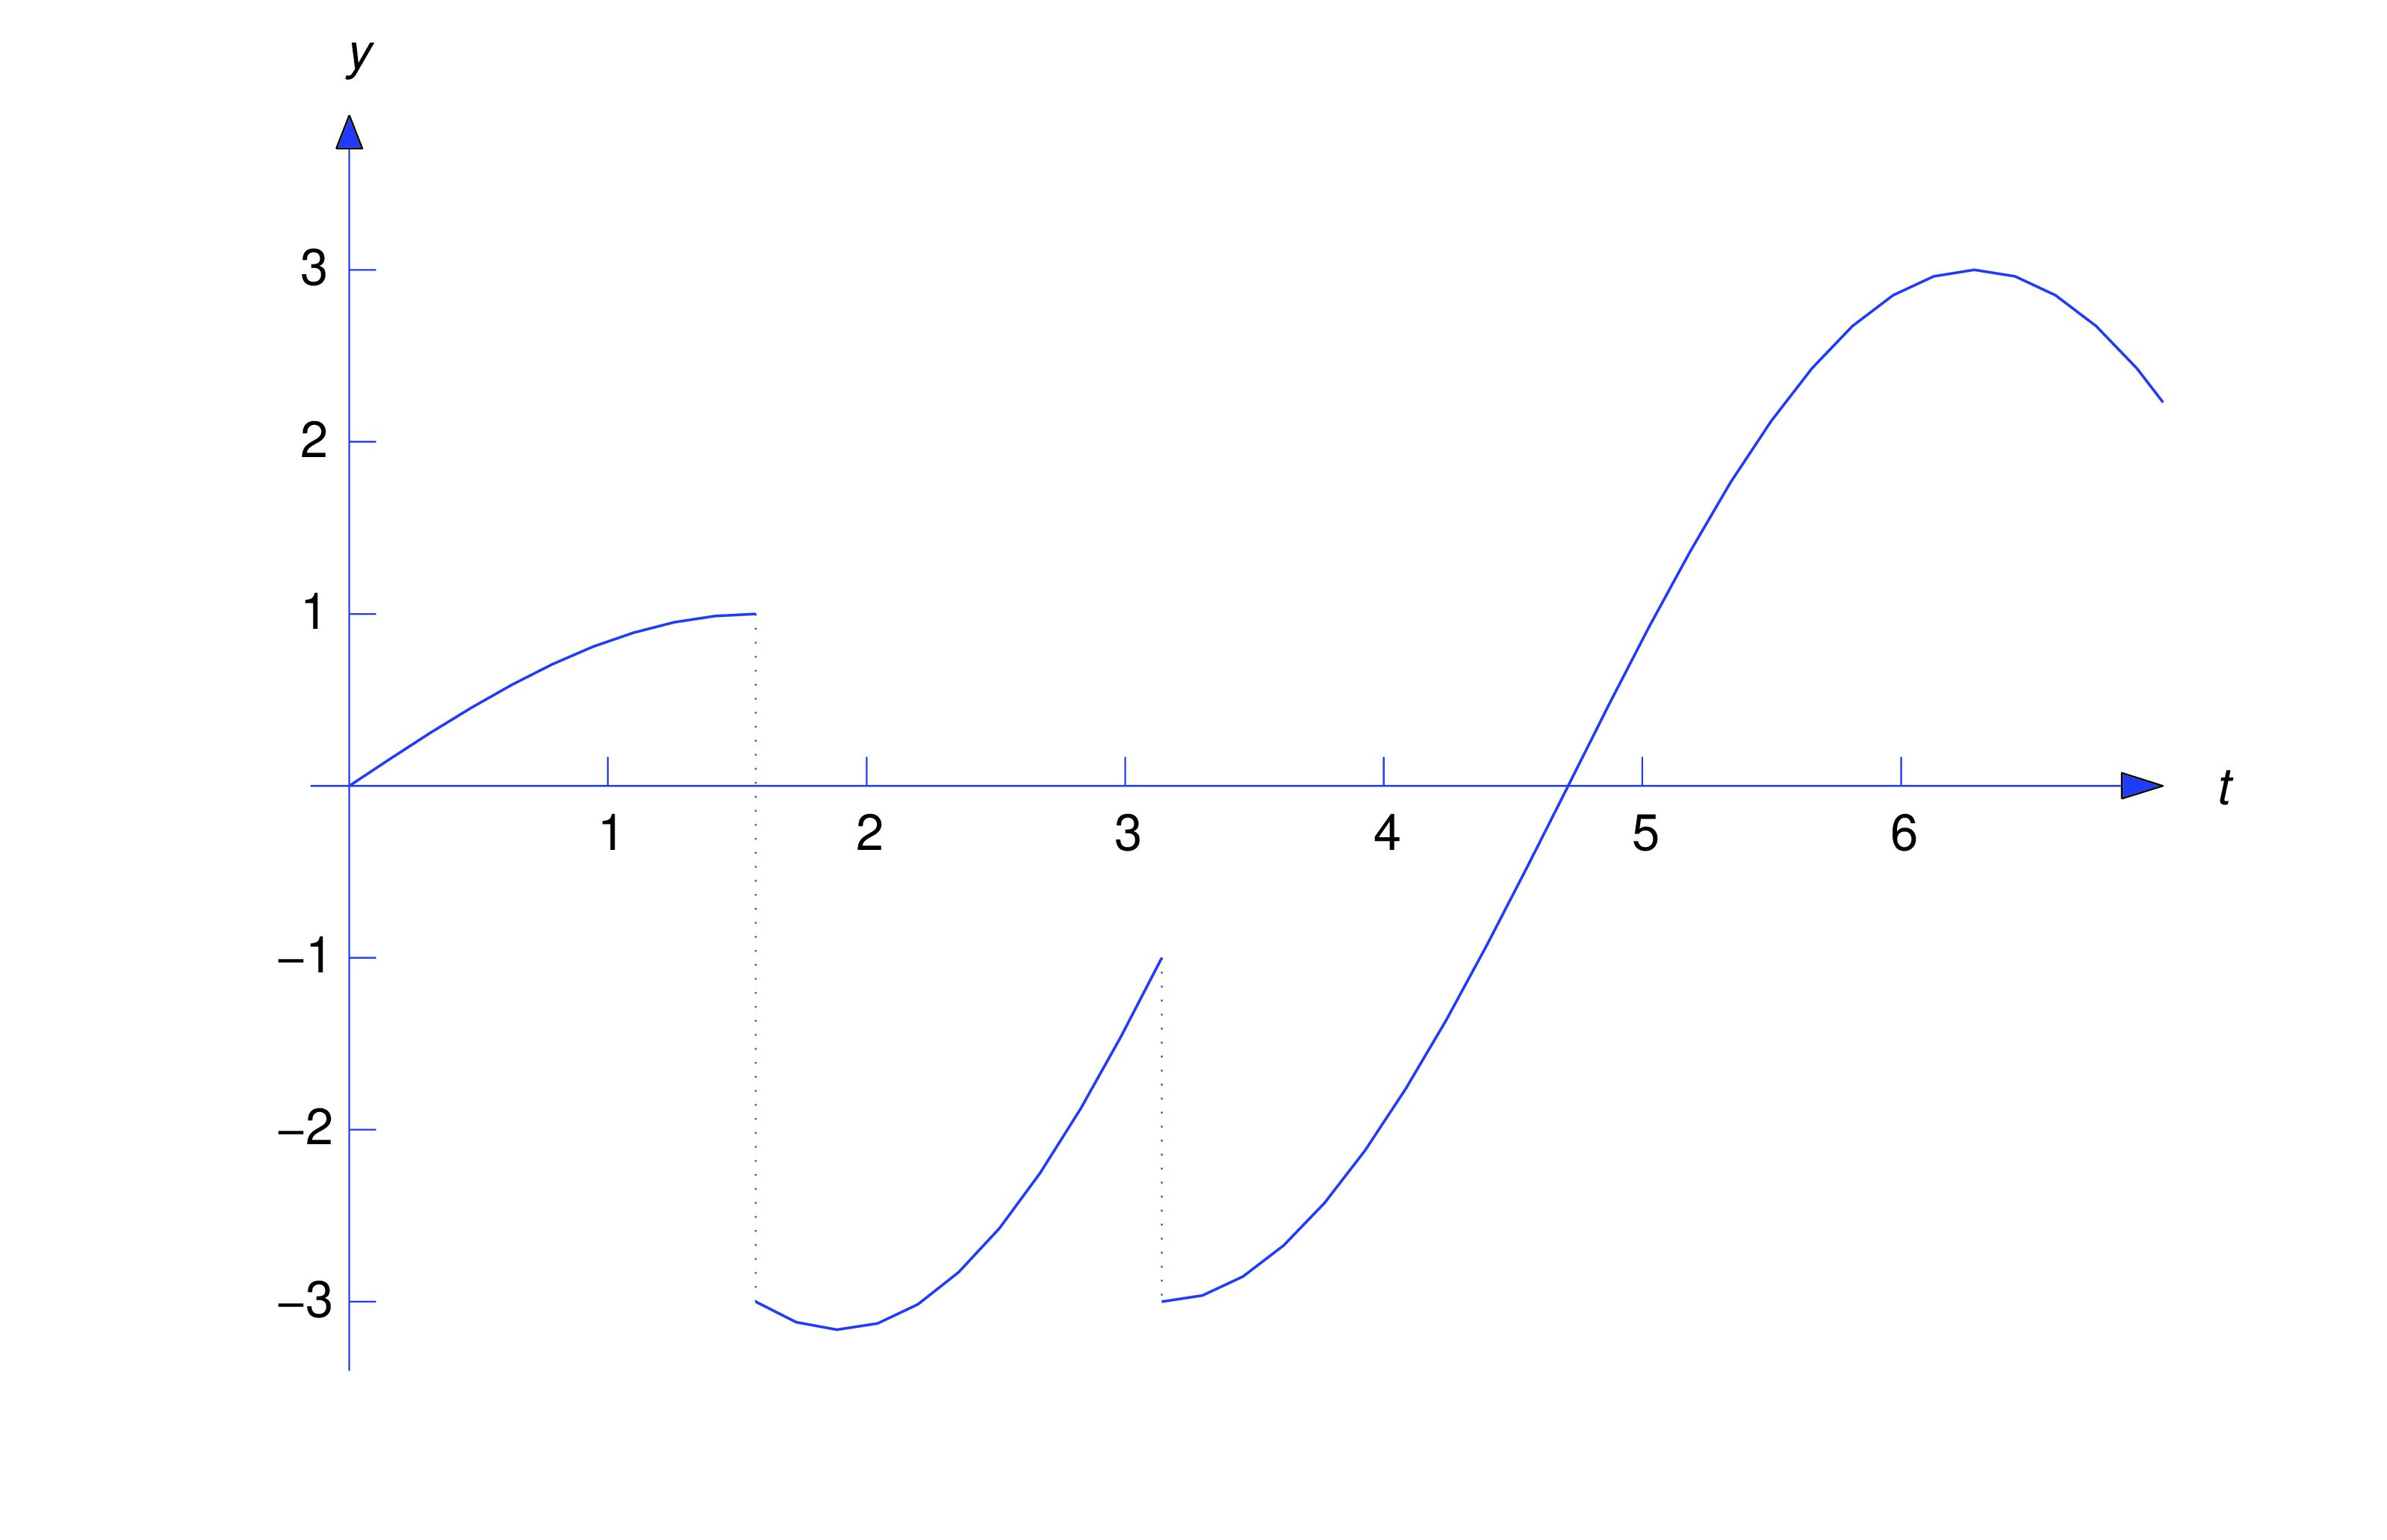
\includegraphics[height=1.5in]{fig080404.jpg}
 \end{image}
%(Figure~\ref{figure:8.4.4}).
\begin{explanation}
In terms of step functions,
$$
f(t)=\sin t+u(t-\pi/2) (\cos t-4\sin t)+u(t-\pi) (2
\cos t+3\sin t).
$$
Now Theorem~\ref{thmtype:8.4.1} implies that
\begin{equation}\label{eq:8.4.11}
\begin{array}{ccl}
{\cal L}(f)&=&{\cal L}(\sin t)+e^{-\pi s/2}{\cal L}
\left(\cos\left(t+\frac{\pi}{2}\right)-4\sin\left(t+\frac{\pi}{2}\right)\right)\\
&&\qquad+e^{-\pi s}{\cal L}\left(2\cos(t+\pi)+3\sin(t+\pi)\right).
\end{array}
\end{equation}
Since
$$
\cos\left(t+\frac{\pi}{2}\right)-4\sin\left(t+\frac{\pi}{2}\right)=-\sin t-4\cos t
$$
and
$$
 2\cos (t+\pi)+3\sin (t+\pi)=-2\cos t-3\sin t,
$$
we see from \eqref{eq:8.4.11} that
\begin{eqnarray*}
{\cal L}(f)&=&{\cal L}(\sin t)-e^{-\pi s/2}{\cal L}(\sin t+4\cos t)
-e^{-\pi s}{\cal L}(2\cos t+3\sin t)\\
&=&\frac{1}{s^2+1}-e^{-\pi s/2} \left(\frac{1+4s}{s^2+1}\right)
-e^{-\pi s}\left(\frac{3+2s}{s^2+1}\right).
\end{eqnarray*}
\end{explanation}
\end{example}

%                  %
% \begin{figure}[tbp]
%   \centering\color{blue}
%   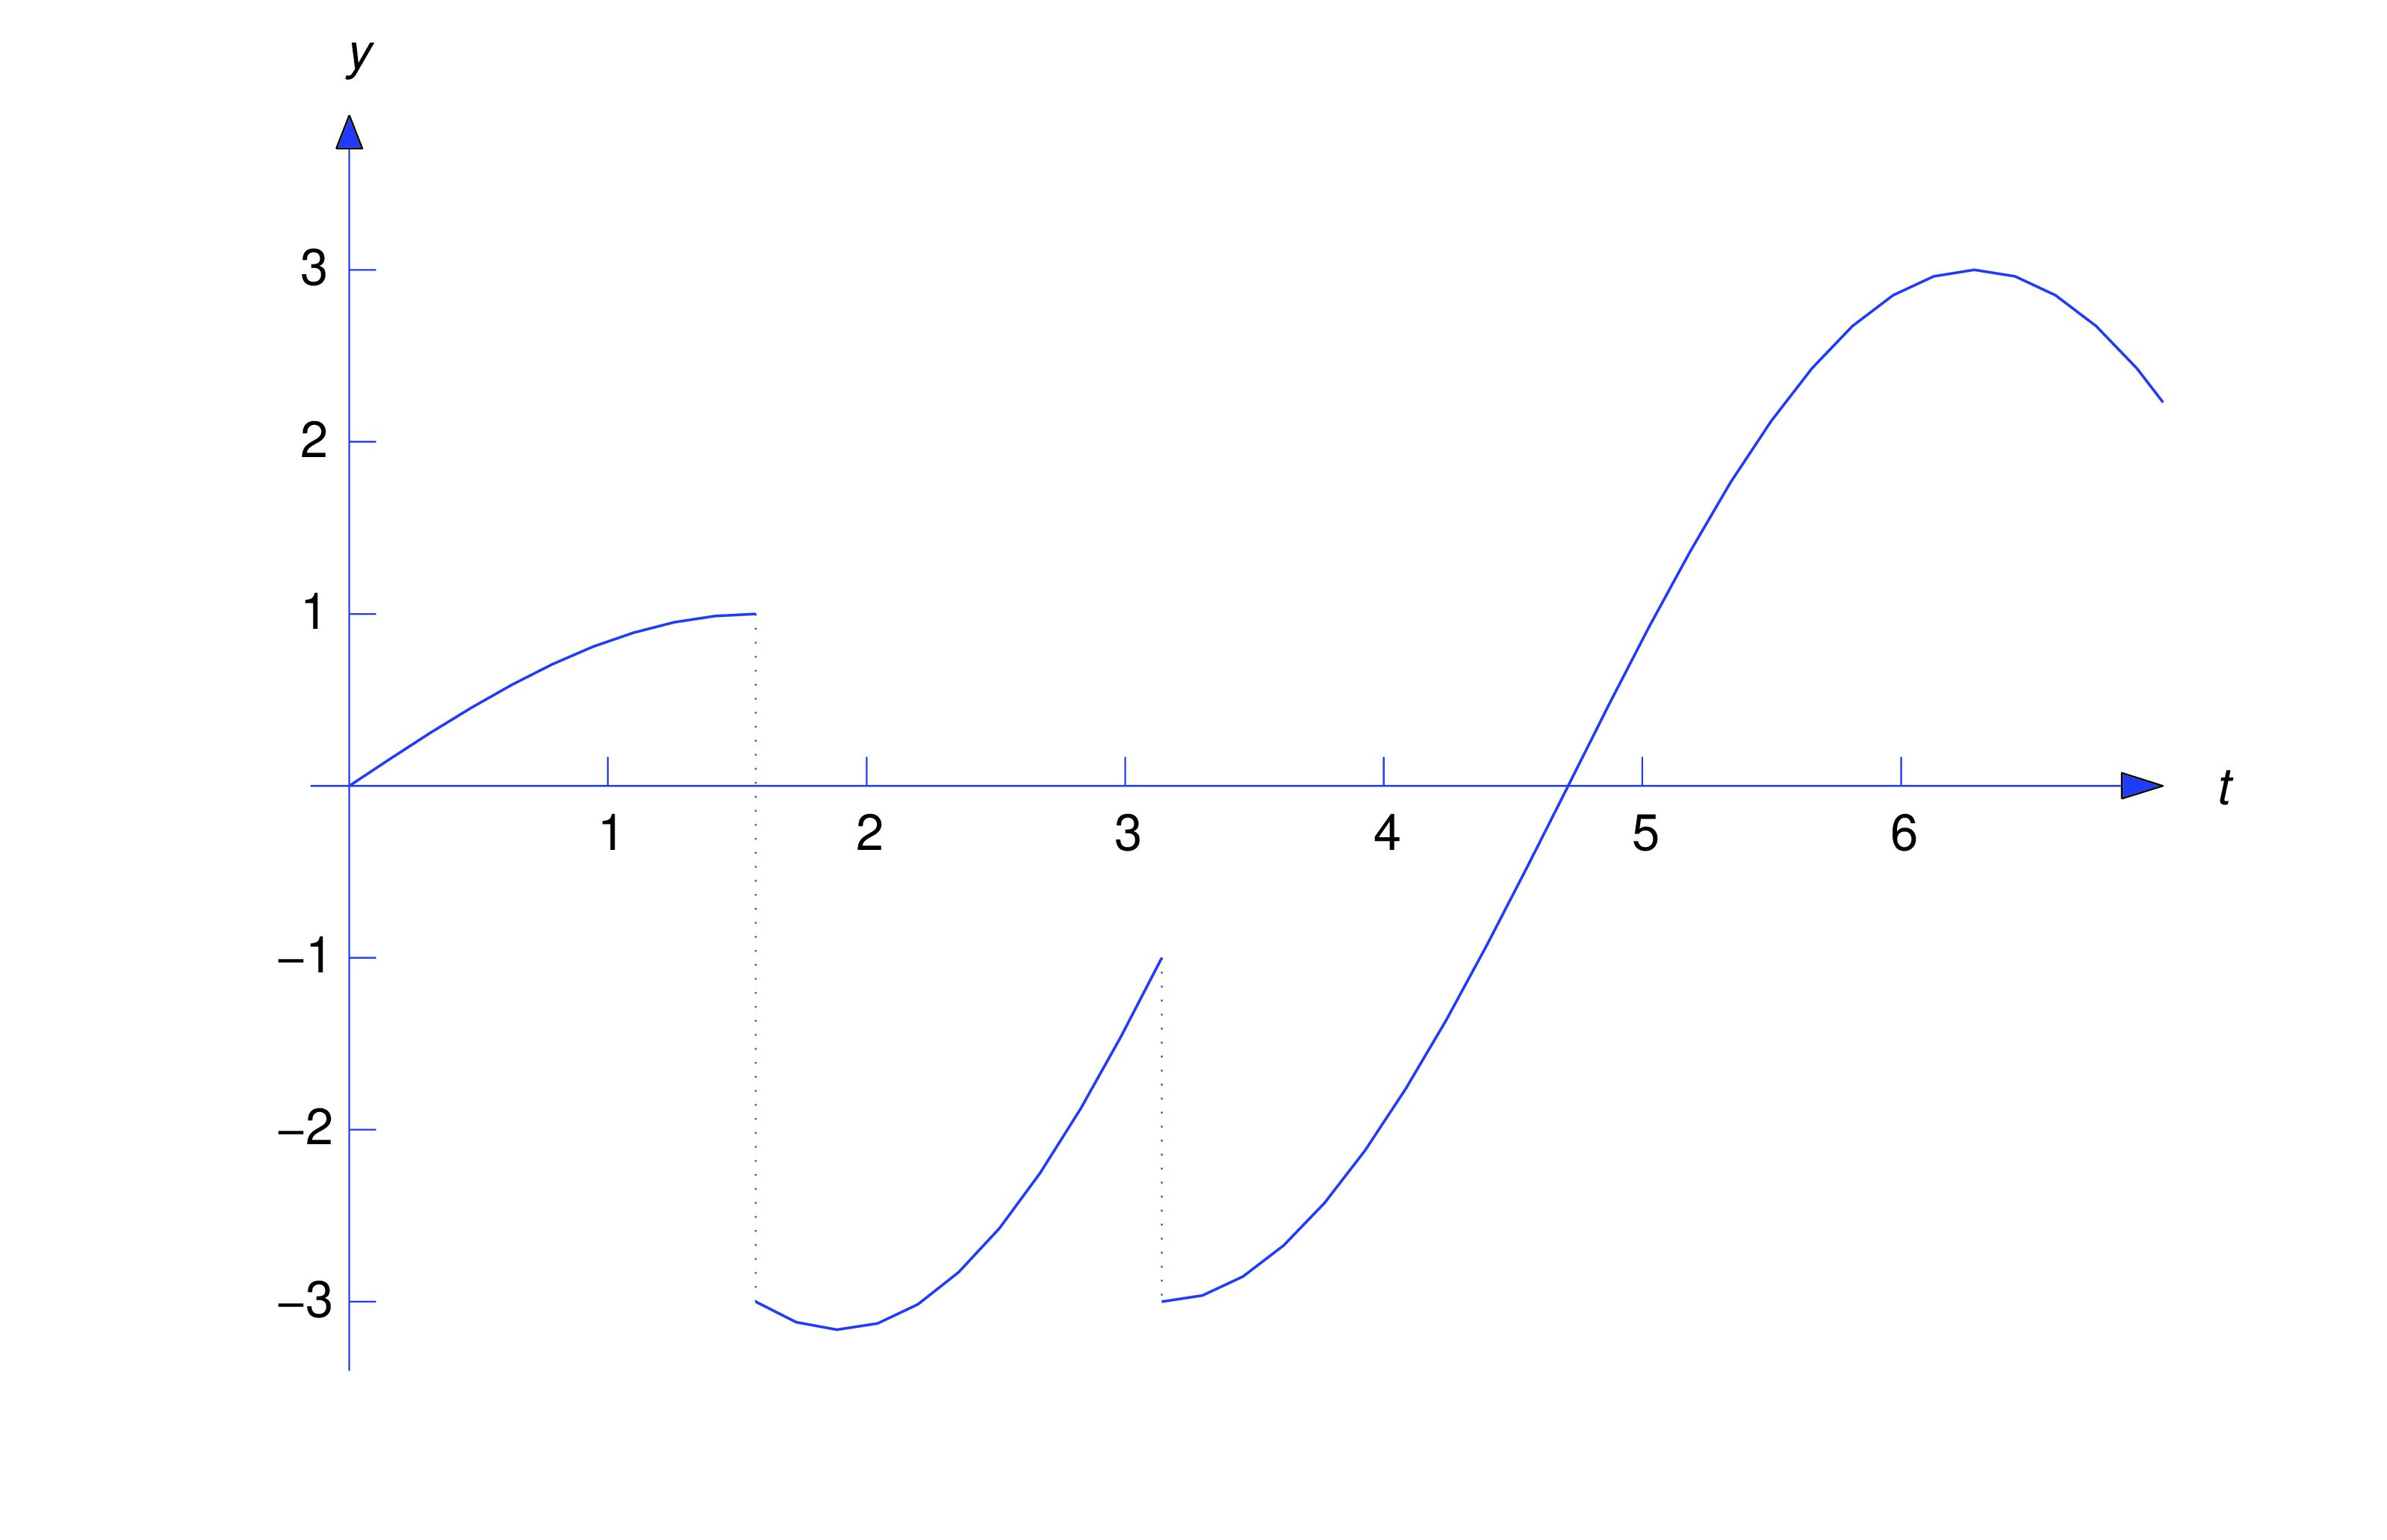
\includegraphics[bb=-78 148 689 643,width=5.67in,height=3.66in,keepaspectratio]{fig080404}
%   \caption{The piecewise continuous function \eqref{eq:8.4.10}}
%   \label{figure:8.4.4}
% \end{figure}



\subsection*{The Second Shifting Theorem}

Replacing $g(t)$ by $g(t-\tau)$ in Theorem~\ref{thmtype:8.4.1}
yields the next theorem.

\begin{theorem}Second Shifting
Theorem]\label{thmtype:8.4.2} If
 $\tau\geq 0$ and ${\cal L}(g)$ exists for $s>s_0$
then  ${\cal L}\left(u(t-\tau)g(t-\tau)\right)$ exists for $s>s_0$ and
$$
{\cal L}(u(t-\tau)g(t-\tau))=e^{-s\tau}{\cal L}(g(t)),
$$
or, equivalently,
\begin{equation}\label{eq:8.4.12}
\mbox{if } g(t)\leftrightarrow G(s),\mbox{ then
}u(t-\tau)g(t-\tau)\leftrightarrow e^{-s\tau}G(s).
\end{equation}
\end{theorem}

\begin{remark}
Recall that the First Shifting Theorem
(Theorem~\ref{thmtype:8.1.3}) states that multiplying a function  by
$e^{at}$ corresponds to shifting the argument of its transform by $a$
units. Theorem~\ref{thmtype:8.4.2} states that multiplying a Laplace
transform by the exponential $e^{-\tau s}$ corresponds to shifting the
argument of the inverse transform by $\tau$ units.
\end{remark}

\begin{example}\label{example:8.4.6}
 Use \eqref{eq:8.4.12} to find
$$
{\cal L}^{-1}\left(\frac{e^{-2s}}{s^2}\right).
$$
\begin{explanation}
To apply \eqref{eq:8.4.12} we let
$\tau=2$ and $G(s)=1/s^2$. Then $g(t)=t$ and \eqref{eq:8.4.12} implies that
$$
{\cal L}^{-1}\left(\frac{e^{-2s}}{s^2}\right)=u(t-2)(t-2).
$$
\end{explanation}
\end{example}

\begin{example}\label{example:8.4.7}
 Find the inverse Laplace transform $h$ of
$$
H(s)=\frac{1}{s^2}-e^{-s}\left(\frac{1}{s^2}+\frac{2}{s}\right)+
e^{-4s}\left(\frac{4}{s^3}+\frac{1}{s}\right),
$$
and find distinct formulas for $h$ on appropriate intervals.
\begin{explanation}
Let
$$
G_0(s)=\frac{1}{s^2},\quad G_1(s)=\frac{1}{s^2}+\frac{2}{s},\quad
G_2(s)=\frac{4}{s^3}+\frac{1}{ s}.
$$
Then
$$
g_0(t)=t, g_1(t)=t+2, g_2(t)=2t^2+1.
$$
Hence, \eqref{eq:8.4.12} and the linearity of ${\cal L}^{-1}$ imply that
\begin{eqnarray*}
h(t)&=&{\cal L}^{-1}\left(G_0(s)\right)-{\cal
L}^{-1}\left(e^{-s}G_1(s)\right)+{\cal
L}^{-1}\left(e^{-4s}G_2(s)\right)\\
&=&t-u(t-1)\left[(t-1)+2\right]+u(t-4)\left[2(t-4)^2+1\right]\\
&=&t-u(t-1)(t+1)+u(t-4)(2t^2-16t+33),
\end{eqnarray*}
which can also be written as
$$
h(t)=\left\{\begin{array}{cl}
 t,&0\leq t<1,\\
-1,&1\leq t<4,\\
2t^2-16t+32,&t\geq 4.
\end{array}\right.
$$
\end{explanation}
\end{example}

\begin{example}\label{example:8.4.8}
 Find the inverse transform of
$$
H(s)=\frac{2s}{s^2+4}-e^{-\pi s/2} \frac{3s+1}{s^2+9}+e^{-\pi
s}\frac{s+1}{s^2+6s+10}.
$$
\begin{explanation}
Let
$$
G_0(s)=\frac{2s}{s^2+4},\quad G_1(s)=-\frac{(3s+1)}{s^2+9},
$$
and
$$
G_2(s)=\frac{s+1}{s^2+6s+10}=\frac{(s+3)-2}{(s+3)^2+1}.
$$
Then
$$
g_0(t)=2\cos 2t,\quad g_1(t)=-3\cos 3t-\frac{1}{3}\sin 3t,
$$
and
$$
g_2(t)=e^{-3t}(\cos t-2\sin t).
$$
Therefore \eqref{eq:8.4.12} and the linearity of ${\cal L}^{-1}$
imply that
\begin{eqnarray*}
h(t)&=&2\cos 2t-u(t-\pi/2)\left[3\cos
3(t-\pi/2)+\frac{1}{3}\sin 3\left(t-\frac{\pi}{2}\right)\right]\\
&&+u(t-\pi)e^{-3(t-\pi)}\left[\cos (t-\pi)-2\sin (t-\pi)\right].
\end{eqnarray*}
Using the trigonometric identities  \eqref{eq:8.4.8} and
\eqref{eq:8.4.9}, we can rewrite this as
\begin{equation} \label{eq:8.4.13}
\begin{array}{rcl}
h(t)&=&2\cos 2t+u(t-\pi/2)\left(3\sin 3t-
\frac{1}{3}\cos 3t\right)\\
&&-u(t-\pi)e^{-3(t-\pi)} (\cos t-2\sin t)
\end{array}
\end{equation}
\begin{image}
 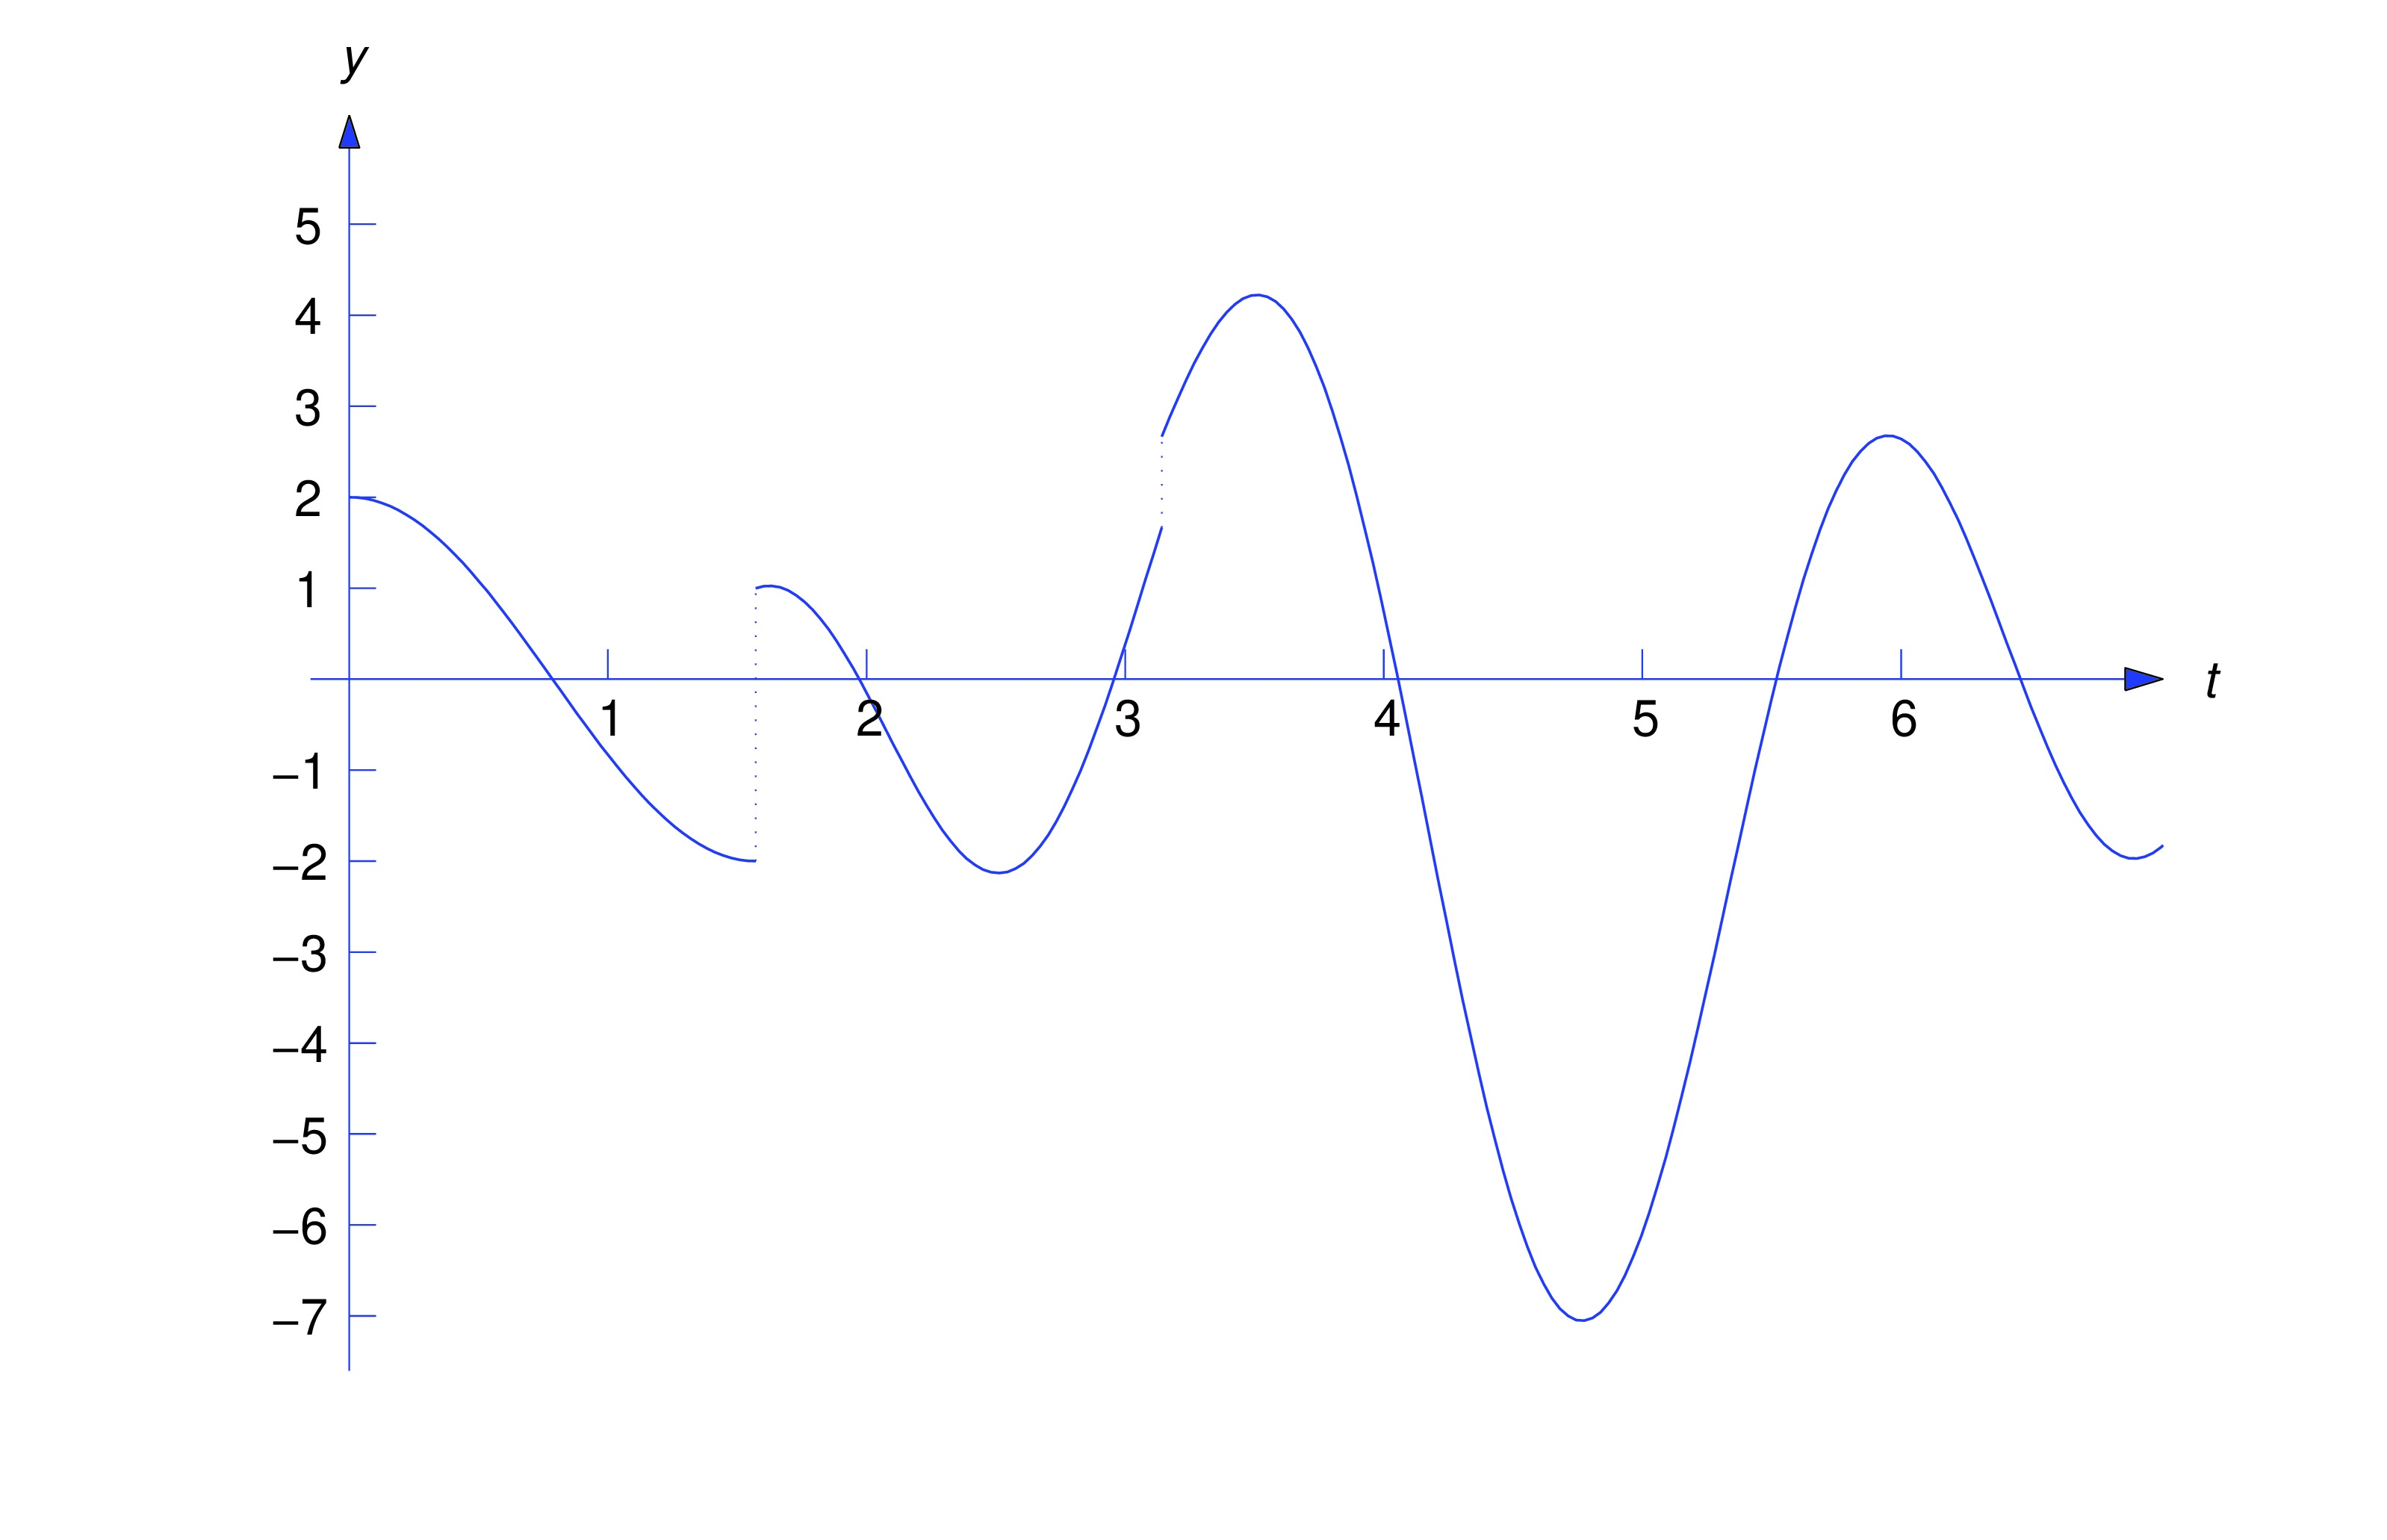
\includegraphics[height=1.5in]{fig080405.jpg}
 \end{image}
\end{explanation}
\end{example}

% \begin{figure}[H]
%   \centering\color{blue}
%   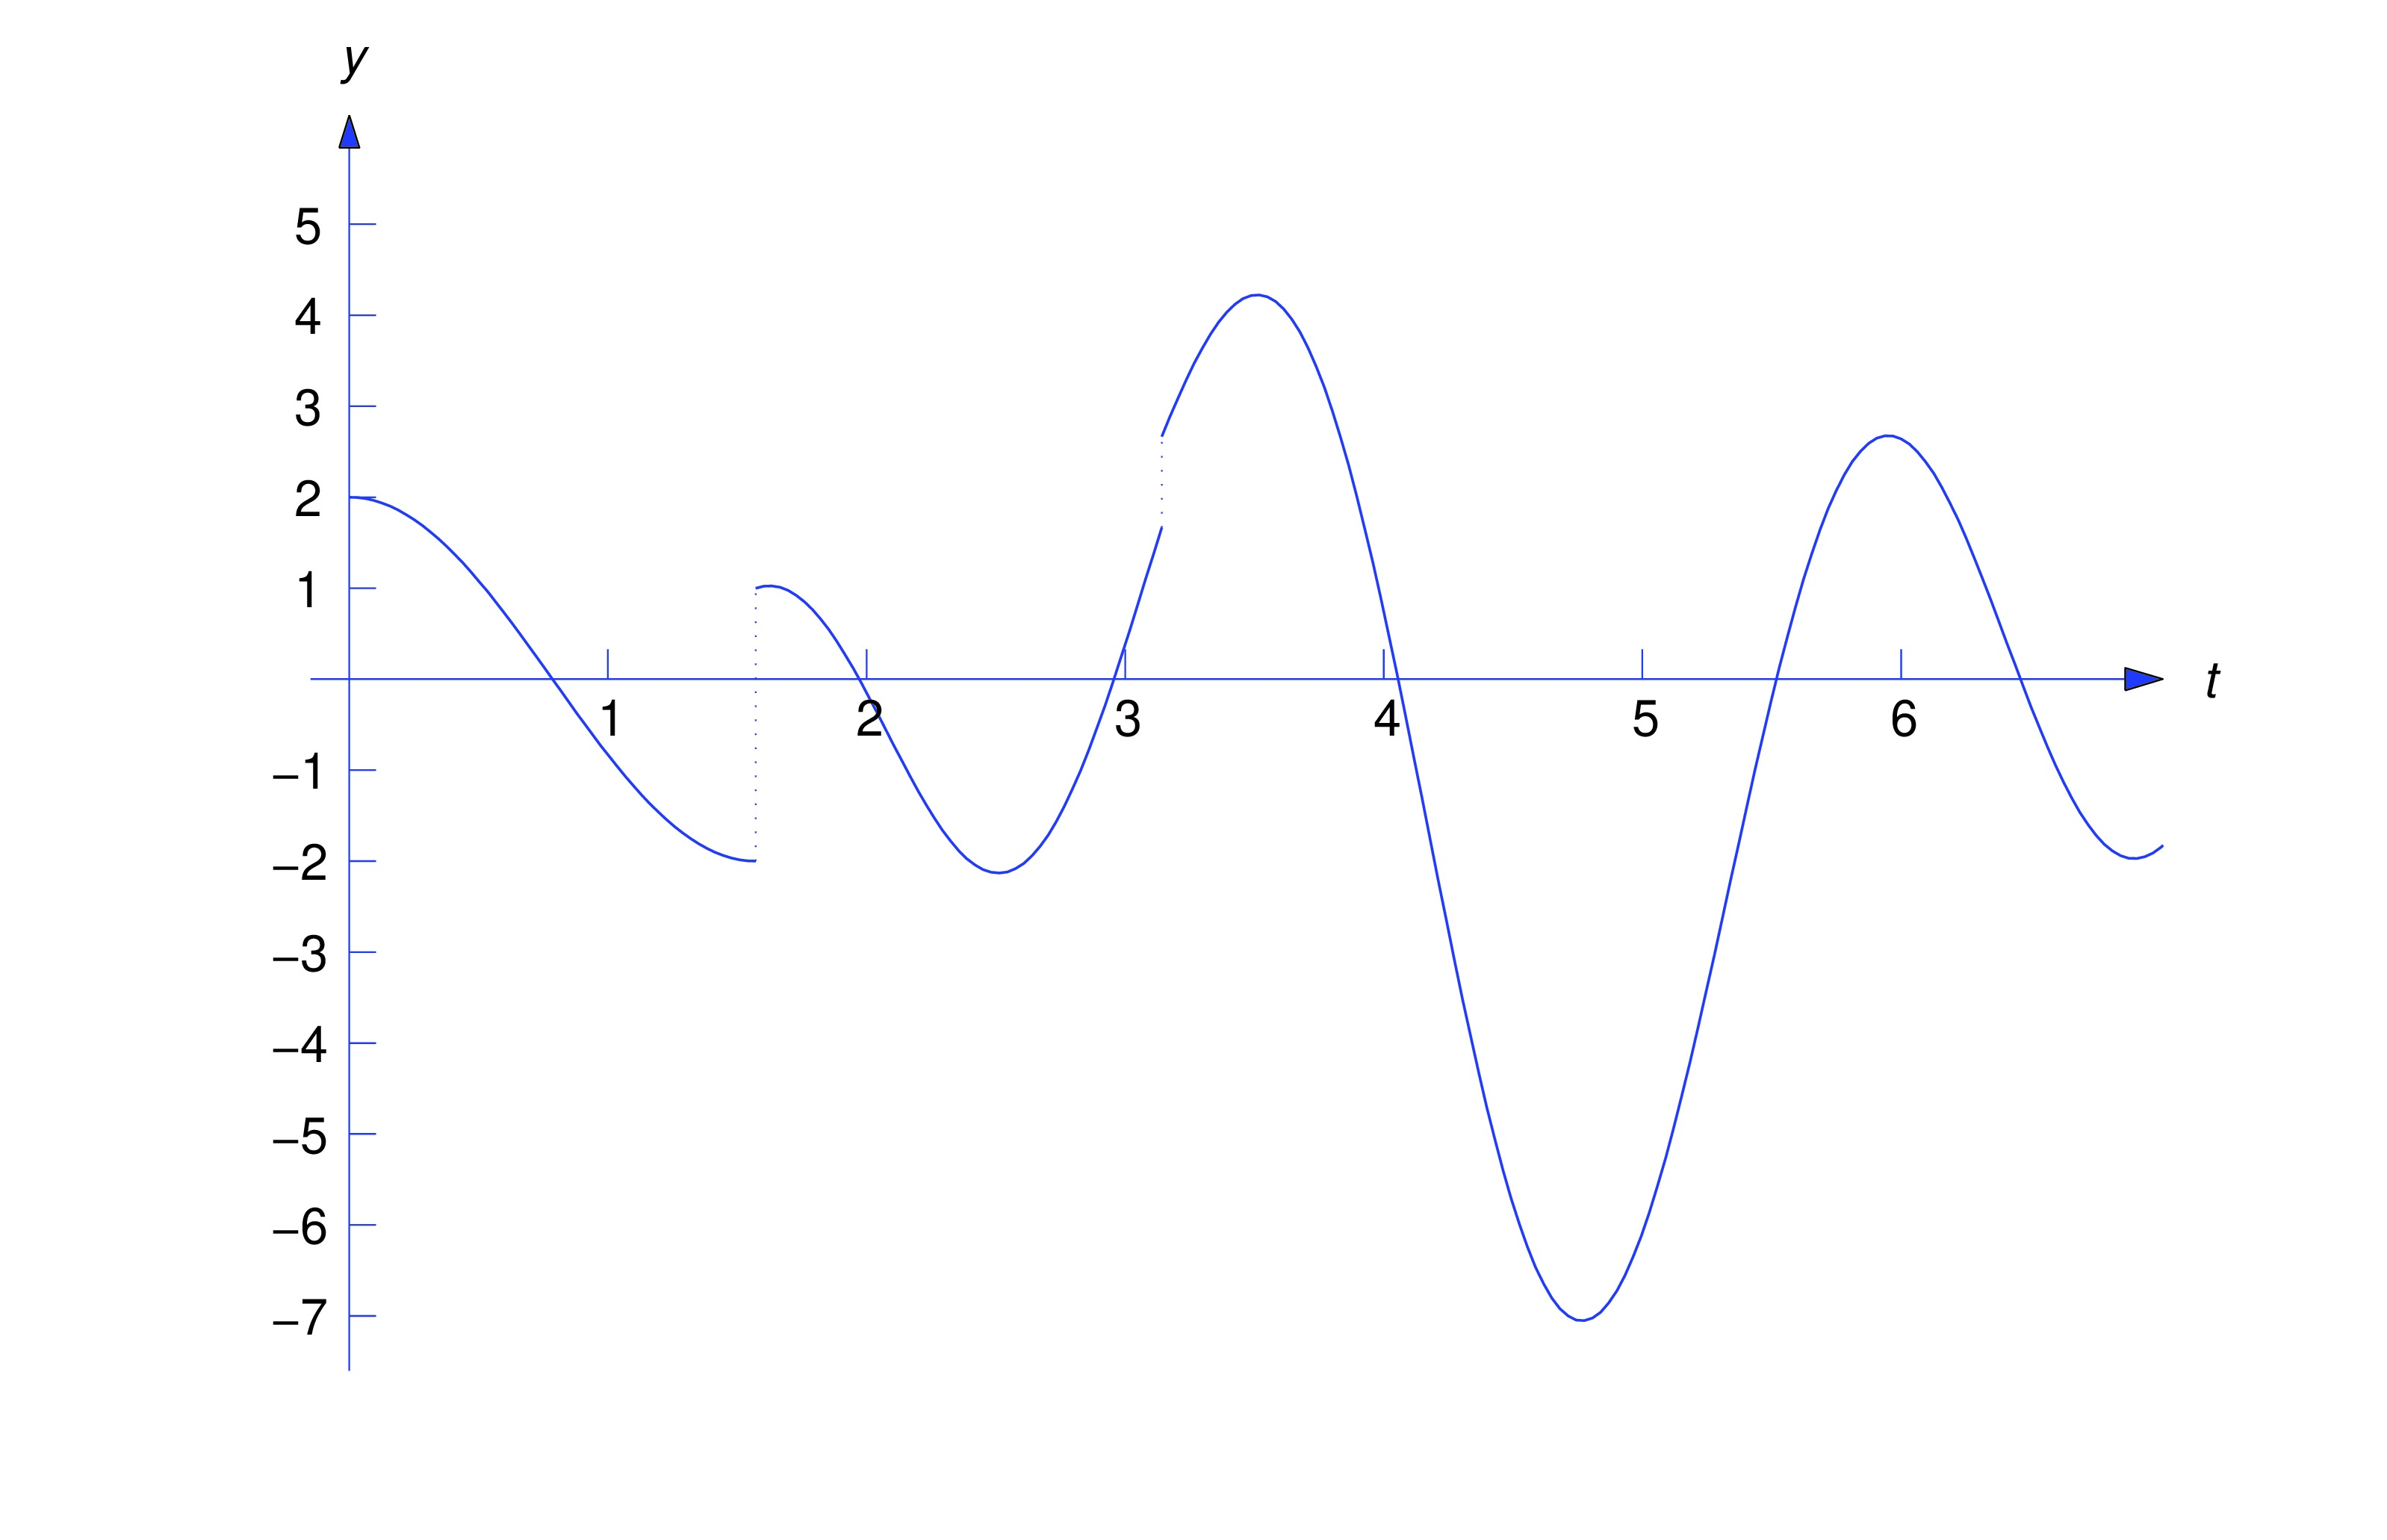
\includegraphics[bb=-78 148 689 643,width=5.67in,height=3.66in,keepaspectratio]{fig080405}
%   \caption{ The piecewise continouous function
% \eqref{eq:8.4.13}}
%   \label{figure:8.4.5}
% \end{figure}

\section*{Text Source}
Trench, William F., "Elementary Differential Equations" (2013). Faculty Authored and Edited Books \& CDs. 8. (CC-BY-NC-SA)

\href{https://digitalcommons.trinity.edu/mono/8/}{https://digitalcommons.trinity.edu/mono/8/}


\end{document}